\chapter{Instrument Suite}

* Total mass and power requirement

* What do we want to measure and why? Explain why some instruments were picked and some were discarded (we can use the notes from when we did that in class)


\autsection{Sample up-concentration \& injection}{Morten Lykke Hilligsøe}\label{sec:water_flow}
Although the instruments selected for the mission have high detection rates, up-concentration of the surrounding waters will enable the detection and quantification of low concentration compounds. To do this, the surrounding water is passed through a ceramic nano filter, which retains any microbes such as bacteria and viruses, as well as most particles. The filter was originally developed in collaboration with NASA, for use in water recycling systems on space missions. After running the surrounding water through this filter for an extended period of time, the water flow is reversed and directed to the instrument suite. When reversing the water flow, the particles on the surface of the filter will be extracted relatively quickly, thereby resulting in an up concentrated sample liquid.

In order to reverse the water flow, a pump is needed. Peristaltic pumps are mechanically very simple and reliable, and therefore suitable for space missions. However the HPLC system described in section \ref{sec:hplc}, requires a pump operating at pressures outside the range of most peristaltic pumps. In order to combine the two pumps of the filtration system and HPLC system, a single high pressure pump \cite{hplc_motor} is used. The suggested high pressure pump has a maximum flow rate of 40ml/min at 500 psi, and most likely higher at lower pressures. 40ml/min isn't a lot, but it accumulates to 57,6l of water per day. If 50l of water is filtered in 1 day, and the filter residue can then be extracted into 50ml of sample water, an up-concentration factor of 1000 has been achieved, which should be sufficient for most experiments.

To direct the water flow several valves will also be required. Figure \ref{fig:filter} presents a water filtration system, complete with valves and tubing, which can be implemented inside the penetrator, allowing up-concentration of the surrounding water. In this system, a disk-shaped filter is used in combination with a central valve which open or blocks the water flow into the instrument suite, as well as a system of valves (flaps) which opens or blocks external water flow to up-concentrating side of the filter. After the sample reaches the instrument suite, other valves can direct which specific instruments should receive the sample.

\begin{figure}[htb]
	\centering
	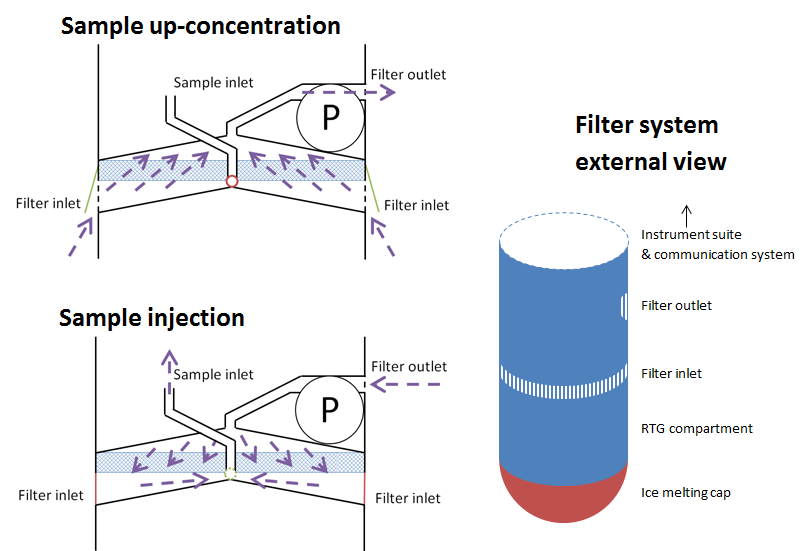
\includegraphics[width=\textwidth]{figures/mlh/filter_multi.PNG}
	\caption{}
	\label{fig:filter}
\end{figure}

A different filtration system was also investigated, in which a pump and a flat filter is used to up-concentrate particles on the surface of the filter, and a mechanical scraper is then used to scrape the surface of the filter, thereby collecting a high concentrate sample. Although a simple solution, the mechanical parts of the scraper might prove less durable than simple valves, and may also end up damaging the filter during operation. 

\autsection{Robot Arm}{Rasmus Lundby Pedersen} % Rasmus
%\chapterauthor{Rasmus L. Pedersen}
Sample manipulation, and extraction, is a central part of lander-based extraterrestrial space exploration. Remote sensing measurements are usually based on non-intrusive observations done at large distances, but it's sometimes necessary to get up and close to the subjects of interest for certain types of material analysis. When measuring factors like temperature, salinity and pH values of a material, close proximity is required and this can either be accomplished by moving all, or part, of the instrument suite close to the sample, or by extracting it to a typically larger central-based instrument laboratory. This section covers the design of a robotic sample manipulator that can achieve both scenarios.

\subsection{Considerations and Drivers}
There are several assumptions that are critical to the design of the robotic sample manipulator. These include, but are not limited to:
\\ 
\begin{itemize}
\item \textbf{High pressure environment}. The manipulator arm is presumably attached to the side of the penetrator, and will be deployed when the vehicle penetrates the bottom of the ice-crust. The common assumption is that the penetrator will experience around 12MPa of pressure at most, but this value may be as high as 36MPa in an absolute worst-case scenario\footnote{$P=\rho g d$, where $\rho\approx 0.92\,\mathrm{kg\cdot m^{-3}}$ for ice-water, $g\approx 1.314\,\mathrm{m\cdot s^{-1}}$ is the approximate gravitational acceleration at Europa's surface and $d=\,30\mathrm{km}$ is the assumed upper limit of the ice-crust thickness}.
\item \textbf{Possible salt-rich water environment}. Material selection should take possible salt-water corrosion into account, since it could be a potential mission-killer.
\item \textbf{Mechanical robustness}. The existence of currents and possible turbulence in the water underneath the crust is currently unknown, and thus is it necessary to design for what could be a very violent marine environment. 
\end{itemize}
These assumption help build a framework of limitations and possibilities for the following instrument suite.
\subsubsection{Sample extraction and reach}
When Earth-based living organisms die and decompose in underwater anaerobic processes, they have shown to form carbon-rich fossil fuels like petroleum and natural gases. These typically exhibit characteristics of having smaller density than water, and will therefore rise to the ice-crust, making the immediate layer underneath the ice an area of interest, with regard to the selection of a sampling location. \\
The samples of interest are most likely liquid, but we must consider the possibility that some organic material are embedded in the ice, due to frequent melting and refreezing of lowest part of the ice-sheet. Therefore, a mechanical element should be positioned at the tip of the manipulator arm so that a small amount of the frozen ice may be dug out, possibly melted by a heating element, and extracted.
\\
\\It must be assumed that the penetrator itself may cause contamination of the surrounding ice when penetrating the crust, as well as introducing a difference in pressure between the water underneath the crust, and the water column melted by the penetrator. The pressure underneath the ice will likely be higher than the pressure in the water column due to possible turbulence, and may suck up a lot of the material located just around the entry-hole. The exact size of the affected area is almost completely unknown since it depends on a myriad of factors, but an approximate reach of $1\,\mathrm{m}$ away from the penetrator should enable us to extract undisturbed ice from the ice-ceiling.
\\
\\A small instrument suite should be placed directly in the tip on the arm to measure the water and ice directly, but some of the sample should be extracted and moved to a centralized instrument suite located in the penetrator, due to space restrictions on the arm.

\subsection{Design Considerations}
With the formulation of the overall goal of the manipulator presented, this section will consider the technical considerations of the arm's design.
\subsubsection{Drill Head}
Temperature profiles previously presented for the ice layer shows, that the ice at the boundary of the liquid sea may be just beneath the freezing point of ice. This makes it a lot easier to dig in and serves as a basis for the design of a drill head.\\
There are several methods for drilling in ice, and this is a central point of discussion with regard to the penetrator descent drilling. The advantages and disadvantages was discussed with the focus of optimizing power-coupling to the ice, and prospective solutions included:
\begin{itemize}
\item Mechanical drilling
\item Laser drilling
\item Sputtering
\item Light concentration drilling
\end{itemize}
At first, light concentration can quickly be disregarded at the present depth of several kilometres, since transportation of natural light from the surface clearly isn't a viable effective solution. Artificial light concentration would technically be indistinguishable from laser drilling.\\
\\
Laser drilling and sputtering are both good alternatives, where the ice would be melted and directly extracted to the penetrator's instrument suite. However, this presents the obstacle that the desired sample-water may be diluted by the surrounding naturally-liquid water and defeat the entire purpose of drilling in the soft ice ceiling. One major advantage is that this method wouldn't require the physical support structure mechanical drilling would.\\
\\
Extracting ice samples with a mechanical drill head carries its own problems, since it would both bring considerable weight from the metal materials, and power consumption associated with motorization of the head, as well a structural stability issues. Cutting, or digging, into the ice requires that pressure is applied from the manipulator arm to the ice, which in turn will result in a reactionary force pushing back on the tethered penetrator which the arm is mounted on. However, this may not be a stand-alone problem, since the mobility of the robotic arm will also require stabilizing arms in any case, and thus will that problem be solved.\\
Power coupling to the ice is also relevant, since the required specific cutting energy varies between methods. The subject of specific cutting energy was touched upon in section covering the penetrator drilling, and is a number that tells us how much energy it takes to remove a unit volume of material. The specific cutting energy is for solid arctic ice, according to [Talalay, Pavel G., 2016]\cite{IceDrill}, (590-680$\,\mathrm{MJ\cdot m^{-3}}$) for thermal drills\footnote{Electric thermal coring drilling and hot-point drilling } and (1.9-4.8$\,\mathrm{MJ\cdot m^{-3}}$) for mechanical drills. It's not clear what type of ice the drill methods were tested in, but this is somewhat irrelevant since the relative specific cutting energy between the methods should be more or less independent of the ice's state.\\ 
Tests have shown that a $CO_2$ laser at $10.6\,\mathrm{\mu\cdot m}$ was able melt about $0.8\,\mathrm{mm\cdot s^{-1}}$ in solid ice, with an intensity of about $50\,\mathrm{W\cdot cm^{-2}}$. Converted to specific cutting energy, this gives:
\begin{equation}
E_{s,laser}=10\cdot\frac{50}{0.8}\,\mathrm{J\cdot cm^{-3}}=625\,\mathrm{MJ \cdot m^{-3}}
\end{equation} 
Which is very similar to that of thermal drilling, which lase-drilling would be a sub-set of. Therefore, it seems that mechanical drilling would be around two orders of magnitude more efficient than thermal- and laser drilling, without accounting for the efficiency of the motor driving the drill bit. \\
\\
It was mentioned that the extracted samples should be retrieved in liquid form, which the laser drilling method intrinsically does. However, a solution to this with regard to mechanical drilling could be to design the head as a cutting wheel with shovelled teeth that could lead the material to a small tube, that would suck the solid ice in by the use of a peristaltic pump. The isolated solid ice would be melted by a electrical heating element and moved further back to the penetrator instrument suite. \\
It could also be possible to a regular conveyor belt-type drill to extract the solid ice, but digging into the ice would anchor the drill head and reduce mobility during sampling. A wheel-bucket cutter like the one seen on figure \ref{fig:WheelCut}  would be more free to move around, assuming that only a shallow cut into the ice would be required.  
\begin{figure}[htb]
	\centering
	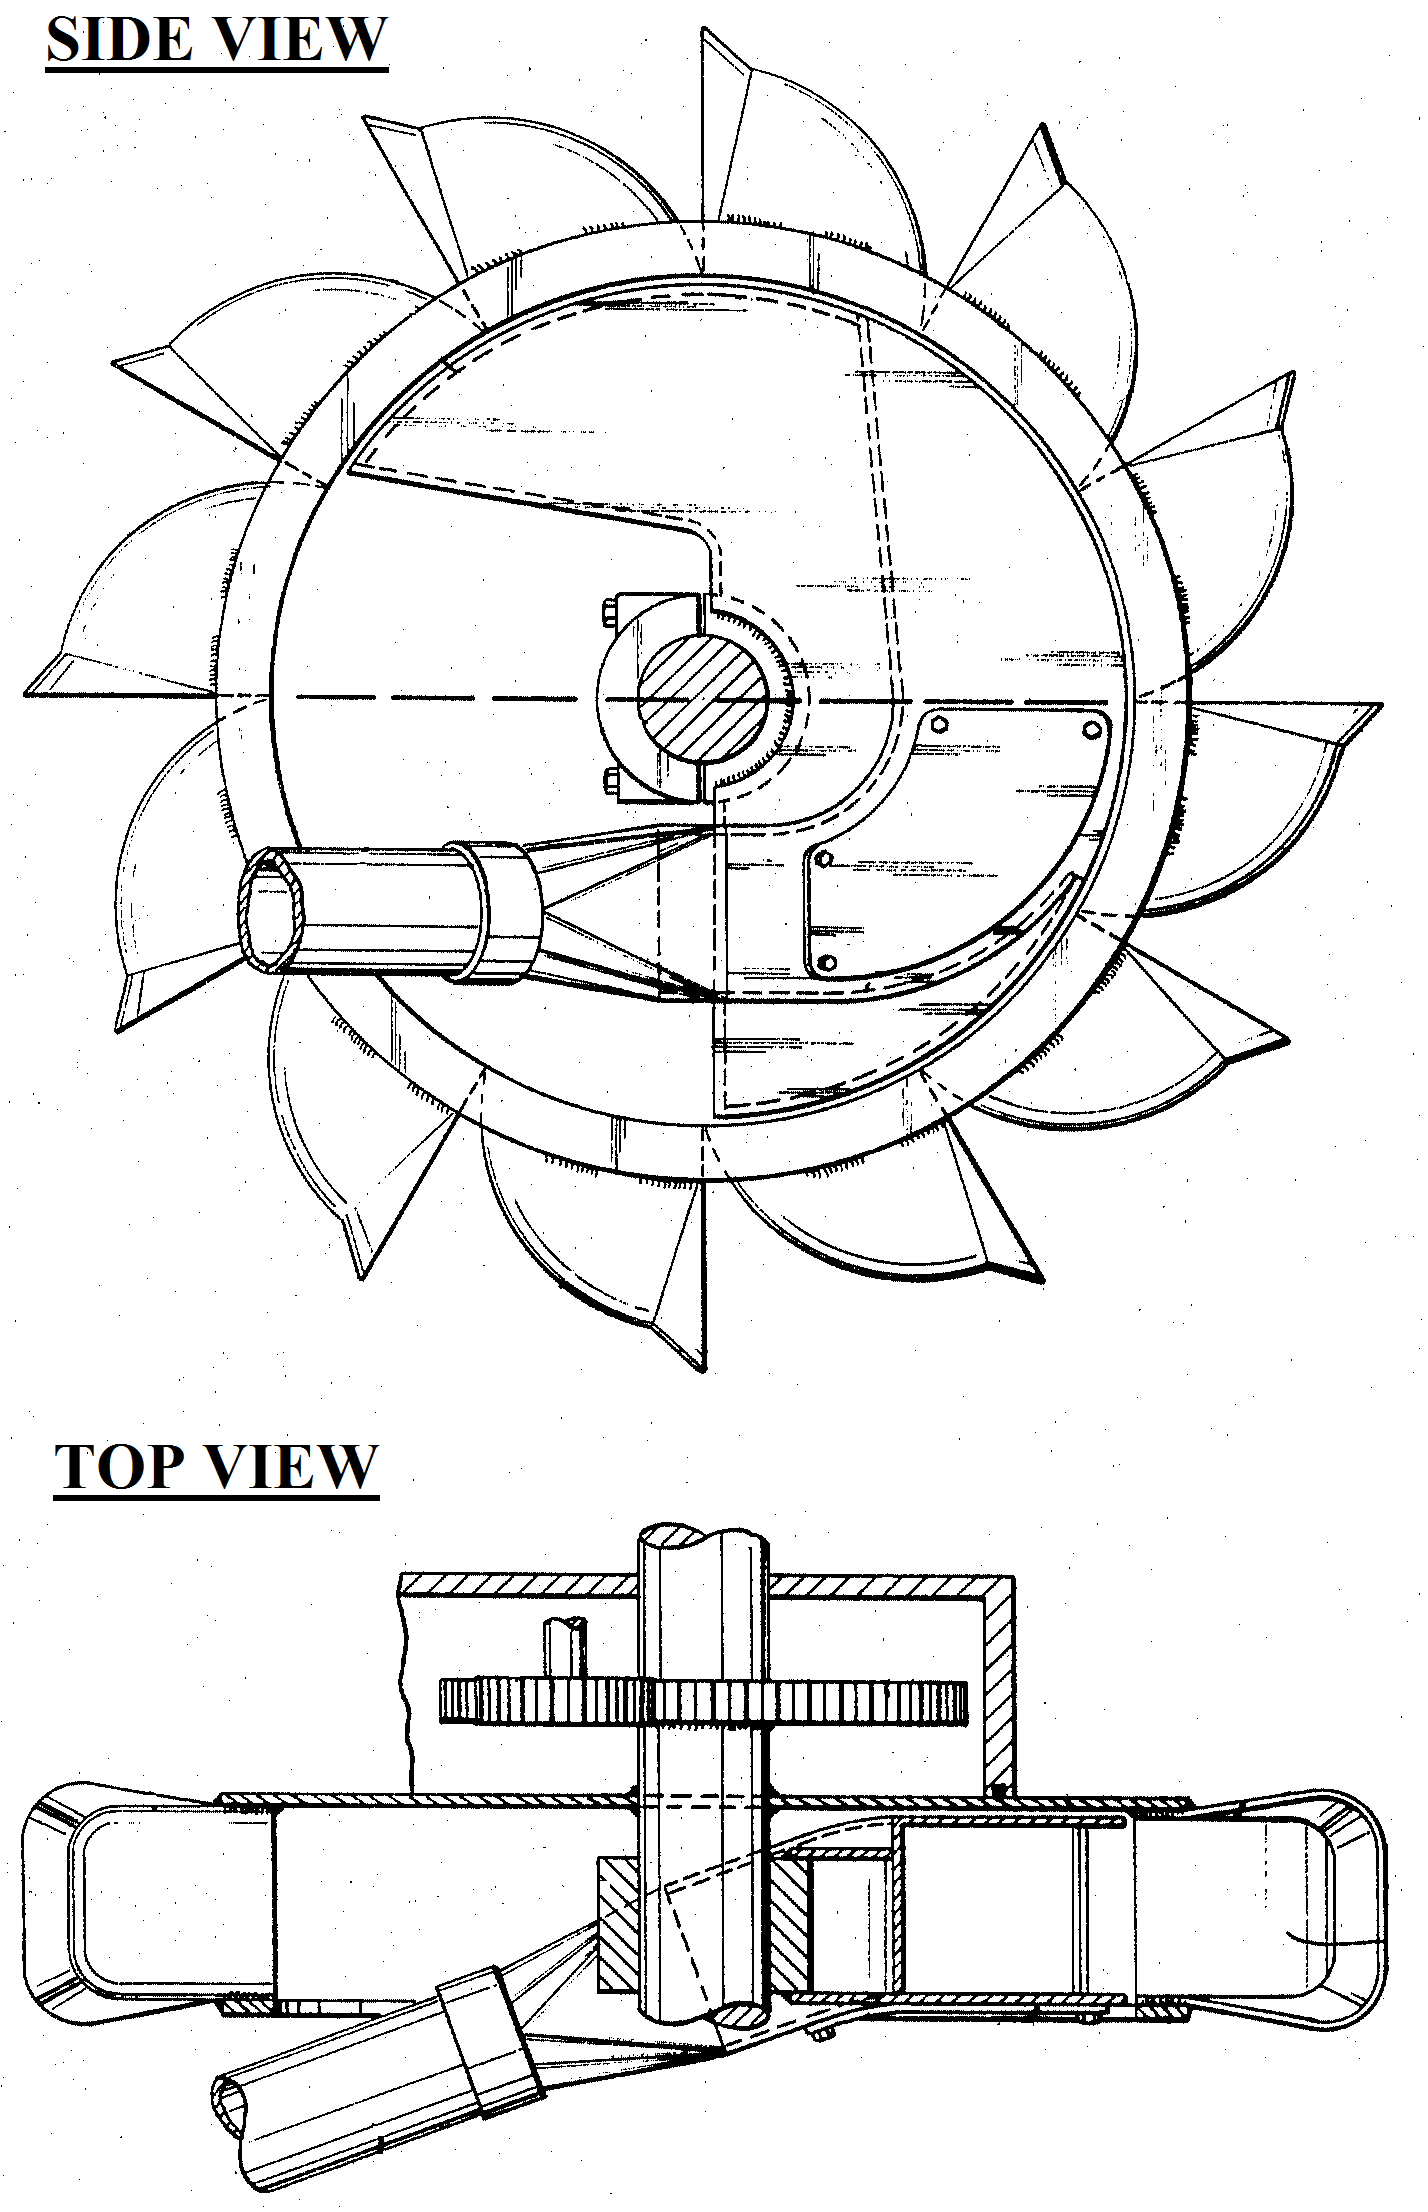
\includegraphics[width=0.35\textwidth]{figures/Rasmus/WheelCutter}
	\caption{Bucket-Wheel cutter design \cite{Vonbucket}.
	\label{fig:WheelCut}}
\end{figure}
\\Selection of wheel-drill material both depends on the required hardness of the material in compared to what's being drilled in, as well as resistance to galvanic corrosion in electrolyte-rich environments like the potential salt-water of Europa's ocean. Titanium and Platinum are both excellent drill bit materials, but are excessively heavy and expensive for the current situation. We assume that we only have to drill in soft ice just below the freezing temperature of water, and thus is strength not as critical an issue. However, we do want to be covered in case of misinterpretation, leading to us encountering harder ice than anticipated. Drill bits made from \textbf{stainless steel} are commonly found in commercial ice-drilling due to its high strength and relatively high metal nobility\cite{Corrosion}.\\
\\

\subsubsection{The Arm and its Degrees of Freedom (DOF)}
Another design aspect is the number, and complexity of the manipulator arm's joints. The bottom tip of the penetrator will likely be occupied by the RTG heating tip used for melting through the ice, so the robot arm should be mounted at a small off-set from the tip. The exact dimensions are currently not now, but it's assumed around 10cm from the tip. The final design should take this into consideration. As mentioned before, the reach of the arm should be at least around $1\, \mathrm{m}$ away, normal to the length of the body at the end closes to the ice. It can be assumed that it's possible for the manipulator arm to be folded down alongside the length of the penetrator body during descent, covering around 75\% of the body's length. One option is to design it as a human arm with a shoulder joint mounted $75\,\mathrm{cm}$ from the ice when hanging tethered from the anchor in the ice (The anchoring could be designed so that this height is variable), an elbow joint, and a wrist joint serving as a mount for the drill bit, and a few instruments - possible in a finger configuration where the instrument are extruded away from the wrist joint in individual finger elements. With this set-up, the arm could be folded over once by the elbow joint, giving a maximum length of 1.5m and in turn a reach of\\
\begin{equation}
R_{reach}=\sqrt{(1.5\,\mathrm{m})^2-(0.75\,\mathrm{m})^2}=1.3\,\mathrm{m}
\end{equation}
Which is sufficient with regard to the requirement of $1,\mathrm{m}$.\\
We are not expecting large variances in the ice composition around the penetrator, which limits the requirement of mobility, since it means we only need to extend the arm straight away from the body. Therefore, are we assuming that no more than one DOF is needed for either the shoulder or elbow joint. The "wrist" joint at the end of the arm, where the drill and an few instruments would be placed should, however, have two DOF's in order to adapt to the possibility of the ice-ceiling being a non-smooth surface with a varying landscape. Pressure sensors mounted on either side of the drill bit could help determine whether the manipulator is in contact with the ice or not, and perhaps help roughly mapping the ice locally around the tip of the arm.\\
\\
As mentioned earlier, the mobility of the arm and the reactionary forces from cutting in the ice, would result in stability issues for the penetrator. Therefore, stabilizing arms should be mounted on the body of the penetrator. One possibility is having one spring-loaded arm mounted directly adjacent (180$^\circ$ around the body) to the manipulator, and two arms located 90$^\circ$ around the body from the first stabilizing arm and the manipulator, directly adjacent to each other.\\
These would, like the robot arms, be folded to the side of the penetrator and released by spring-loaded joints when the penetrator has reached the desired altitude with respect to the ice-ceiling. They should be mounted at the same height of the penetrator body as the manipulator arm and would be extended in a 45$^\circ$ angle from the body when deployed. With a total length of $l_{support}=\frac{0.75\,\mathrm{m}}{cos(45^\circ)}=1.06\,\mathrm{m}$, the tips of the arms would then dig into the ice if the penetrator was to be moved by either water-turbulence or the pushing from the drill bit on the manipulator.


\subsubsection{Autonomy}
Deep-sea remotely operated underwater vehicles (ROV) are usually, as the name suggests, controlled remotely with a live video feed, which is an advantage when investigating unknown sites, underwater structures and animal life. This is primarily due to the need for being able to adapt to the conditions surrounding the ROV. However, this is not possible for the Europa exploration mission, because of the extremely short communication windows and relay times between the penetrator and Earth. The manipulator arm must therefore be autonomous, to a level where it's able to locate, measure and harvest samples by itself when commanded to do so. 

%\subsubsection{Material Extraction}

\subsubsection{Neutral Buoyancy}
Remotely Operated Underwater Vehicles (ROV) used Earth-based are usually designed to have neutral buoyancy in the water. This gives ROV significantly more manoeuvrability, since the its thrusters won't have to work against the gravity of Earth, due to its ability to free-float in the water. The same criteria is desirable for the manipulator arm on the Europa ice-penetrator, with regard to joint stability and power usage of their actuators. With the arm being buoyancy neutral, the only requirements of the joints in terms of power stems from the desired rotational velocity of the shoulder, elbow and wrist joints, which in turn is dependent of the mass of the arm, the instruments mounted on the wrist joint, and the drill at the tip.\\
The general method of obtaining neutral buoyancy is by distributing a material with a density significantly lower than that of water, around the object of interest (desirably above the center of mass for stability considerations). For the arm, the weight isn't distributed uniformly along its length, so neither should the buoyancy material be.\\
Syntactic foam has been widely used and tested for deep-sea high-pressure sea environments. Briefly explained, syntactic foam is a composite material synthesized by infusing a material with hollow gas-containing microballoons. This creates a material with lower overall density and often higher specific strength, which is specifically useful for applications including but not limited to:
\begin{itemize}
\item Deep-sea buoyancy foams.
\item Accoustically attenuating materials.
\item Blast mitigating materials.
\end{itemize}
The strength and low density of the syntactic foam makes it ideal for deep-sea neutral-buoyancy ROV designs, and is therefore worth considering for the penetrator manipulator arm.\\
As mentioned earlier, the expected amount of pressure underneath the ice-ceiling is around $12\,\mathrm{MPa}$, but the absolute assumed theoretical maximum is $36\,\mathrm{MPa}$ which is the equivalence of approximately $3500\,\mathrm{MSW}$\footnote{$1\, \mathrm{MSW}$ is a non-SI unit roughly equivalent to $1\, \mathrm{bar}$}. The AZ-grade syntactic foam offered by Engineered Syntactic Systems is rated for a depth of $4000\,\mathrm{MSW}$ with a density of $465\,\mathrm{\frac{Kg}{m^3}}$, making it viable as a solution.\\
We currently don't know the behaviour of syntactic foam in vacuum, so the housing of the manipulator arm may have to be pressurized during the travel to Europa.

\subsection{Implementation and Design Specifications}
A solution used for scaling reference is the Schilling Robotics TITAN 4 Manipulator \cite{Titan4}, seen on figure \ref{fig:titan4}, driven by hydraulic at the shoulder and an electrical motor at the elbow and wrist joints.
\begin{figure}[htb]
	\centering
	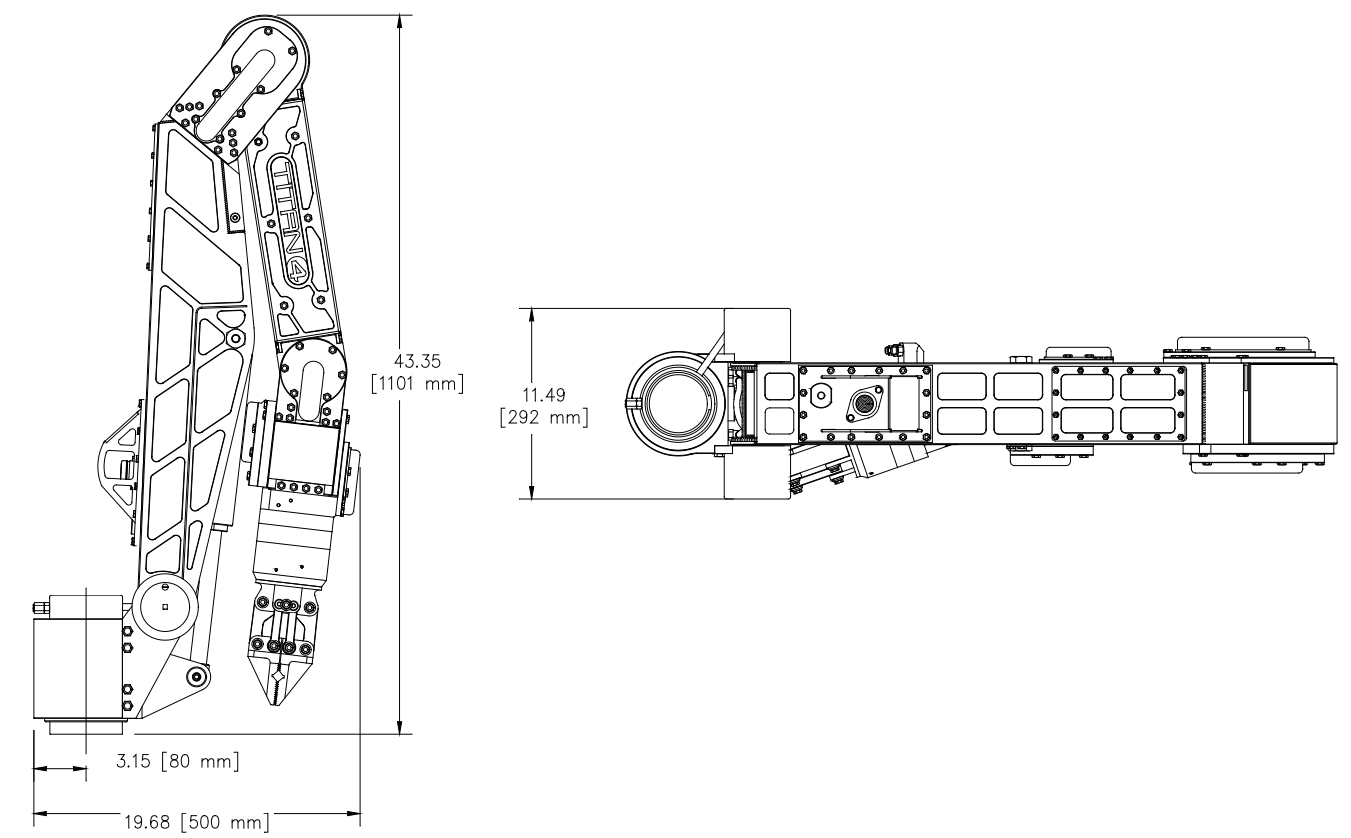
\includegraphics[width=1\textwidth]{figures/Rasmus/Titan4}
	\caption{Titan 4 robotic arm structural drawing, including dimension.
	\label{fig:titan4}}
\end{figure}
 It's made from titanium, and is much larger than the available space on the penetrator, but the relative dimensions and design type can be used for reference. The number of joints, their complexity and individual DOF complies with the mentioned design criterias. However, the manipulator claw at its tip should be replaced by the "hand" consisting of the manipulator wheel-cutter and 2-3 external instruments.\\
The TITAN 4 has a fully extenden arm-length of $2\,\mathrm{m}$, so this could at least be reduced to the required $\mathbf{1.5\,\mathrm{m}}$, $75\,\mathrm{cm}$ per arm section. The storage room for the arm during descent is extremely limited, with the cylinder structure of the penetrator having an outer cross-sectional radius of only $10\,\mathrm{cm}$. Since the penetrator will be filled with other measuring instruments, the arm may only have $300\cdot10^{-3} \,\mathrm{m^3}$ of space, with a folded length of $0.75\,\mathrm{cm}$. This means that the simplified  cross-sectional dimensions must be no more than $2\times 1\,\mathrm{cm}$ (since it would be folded). This is fairly small, and structural analysis on the arm with these dimension would be required for the final solution. From intuition, and not having any experience with mechanical and structual engieering, it does seem like the arm would be too flexible with these dimensions (and movable joints) of $1\times 2\times 150\,\mathrm{cm}$. This may eliminate the possibility of a robotic arm as we want it to be fairly stable in the water.\\ 
The mass of the full-size arm in air is $100\,\mathrm{kg}$, which would make the modified arm alone:
\begin{equation}
m_{arm}=\frac{1.5\,\mathrm{m}}{2\,\mathrm{m}}\cdot\frac{1\,\mathrm{cm}}{30\,\mathrm{cm}}\frac{2\,\mathrm{cm}}{30\,\mathrm{cm}}\cdot 100\,\mathrm{kg}=0.166\,\mathrm{kg}
\end{equation}
Which seems very small. It would also be possible to modify the design, in order to make it more efficient, with regard to storage space. Re-designing the elbow joint so that the arm folds the other way, would make the folded arm more or less flush with the extruding mount, and it could also be possible to make the arm wider, but leave space in its center, so that it could be folded within itself.\\
It is not know how the arms depth rating of $4000\,\mathrm{MSW}$ would be affected by the size scaling, with respect to the hydraulic shoulder joint.\\
\\
Assuming the arm is made solely out of titanium, which has a density of $2700\,\frac{\mathrm{kg}}{\mathrm{m^3}}$, the effective volume of the arm will be 
\begin{equation}
V_{eff,arm}=\frac{m_{arm}}{\rho_{alu}}=\frac{0.166\,\mathrm{kg}}{2700\,\mathrm{\frac{kg}{m^3}}}=61.5\cdot 10^{-6} \, \mathrm{m^3}
\end{equation}
\\
In order for the arm have neutral buoyancy, the gravitational forces on the arms$+$the buoyancy material must cancel out with the buoyancy forces of the two. We assume that the instruments and the drill bit weighs $m_{drill}=2\,\mathrm{kg}$ and has the density of steel with a volume of $V_{drill}=2\times 2 \times 0.5 \, \mathrm{cm}=2\,\mathrm{cm^3}=2\cdot 10^{-6}m^3$. If the volume of the syntactic foam is denounced by $V_{buoy}$, the equation will for the arm in salt water ($\rho_{saltwater}=1029 \, \mathrm{\frac{kg}{m^3}}$) be:
\begin{equation}
\begin{split}
&m_{arm}+V_{buoy}\cdot \rho_{buoy} + m_{drill}=(V_{buoy}\cdot + V_{arm}+V_{drill})\rho_{saltwater}\\
&\rightarrow 0.166\,\mathrm{kg}+V_{buoy}\cdot 465 \mathrm{\frac{kg}{m^3}}+2\,\mathrm{kg}=(V_{buoy}+61.5\cdot 10^{-6}\,\mathrm{m^3}+2\cdot 10^{-6}m^3)\cdot 1027 \,\mathrm{\frac{kg}{m^3}}\\
& \leftrightarrow V_{buoy} = 3.738\cdot 10^{-3}\,\mathrm{m^3}
\end{split}
\end{equation}
Adding more volume to the problem isn't desired, and we may have to conclude that there simply isn't space enough to store the robot arm during descent, for the current design parameters.\\
With the added syntactic foam of $m_{foam}=3.738\cdot 10^{-3} \,\mathrm{m^3}\cdot 465\mathrm{\frac{kg}{m^3}}=1.7382\,\mathrm{kg}$, and the drill head with a few instruments, the arm will weigh and can take up somewhere around:\
\begin{subequations}
\begin{equation}
m_{arm,total}=0.166\,\mathrm{kg}+2\,\mathrm{kg}+1.7832\,\mathrm{kg}=3.95\,\mathrm{kg}
\end{equation}
\begin{equation}
V_{arm,total}=61.5\cdot 10^{-6}\,\mathrm{m^3}+2\cdot 10^{-6}\,\mathrm{m^3}+3.738\cdot 10^{-3}\,\mathrm{m^3}=3.8\,\mathrm{m^3}
\end{equation}
\end{subequations}
Which shows that most of the space will be taken up by the buoyancy material. This can be solved by using a lighter material like steel, but the stiffness of this material may be too low with respect to the structual dimensions of the arm.\\
It's unsure how the power consumption of the motors and control systems scale with size, but they are not expected to use more than $P_{arm}=20\,\mathrm{W}$ in total, when running.\\
A simply estimation of the total mass, volume and power costs of the manipulator arm can be seen on table \ref{tab:Arm}.

\begin{table}[htb]
\centering
	\begin{tabular}{| l | l | l | l |}
	\hline
	\textbf{Unit}	&	\textbf{Weight ($\mathrm{kg}$)}	&	\textbf{Volume  ($\mathrm{m^3}$})	&	\textbf{Power (W)}\\ \hline
	Arm structure + joints	& 0.166	&	$61.5\cdot 10^{-6}$	&	\\ \hline
	Support arm	$\times 3$&	0.5	& $184.5\cdot 10^{-6}$	&	\\ \hline
	Syntactic foam	&	1.78	&	$3.738\cdot 10^{-3}$	&	\\ \hline
	Motors + drivers	&	2	&	$0.1\cdot 10^{-3}$	&	20	\\	\hline
	Drill head	&	0.016	&	$2\cdot 10^{-6}$	&	\\ \hline
	\hline
	Total	&	4.13	&	4	&	20\\
	\hline	
	%
	\end{tabular}
	\caption{Total mass, volume and power costs of the manipulator arm.}
	\label{tab:Arm}
\end{table}
The power and weight costs seem to be within reasonable ranges. 
 

\section{Sample handling}

* We need a design, I (Kristian) talked with some other about this, but we need to coordinate with the rest of the groups
   (SMS http://www.esmats.eu/amspapers/pastpapers/pdfs/2008/mumm.pdf)

* Sample rate

* What is under pressure and what is not?

* Order of the instruments



\autsection{CTD/ADCP}{Jean-Paul Breuer}
CTD (Conductivity, Temperature, Depth) and ADCP (Acoustic Doppler Current Profiler) are two instruments that are very much typical and frequently used in oceanography. The CTD is lowered through the water column taking measurements of the water and creating a profile of the salinity and temperature throughout the column. The ADCP is used for determining the speed and direction of an underwater current. These instruments are important because it is critical to get an understanding of the conditions within the ocean, not only to find life, but to be able to further understand how the system is functioning and coevolving with the tidal wave and orbit around Jupiter. It might even give some interesting data if there are black smokers or any kind of uncommon activity in the area (or which may get dragged past due to the current).

Typically the CTD and ADCP are fairly small and lightweight, but are two separate instruments; however, there was an idea for how to effectively join the two instruments to get the same information and save some space in the instrument suite. To approach the problem by starting with assumptions, the instruments will require to descend through the water column, but to increase the output of data, it would be ideal to reduce the rate of descent while also increasing the sampling area so that there is a larger water column with samples. The idea is to drop the instrument into the water and to have hydrofoils that enable it to glide in large spirals down from the top of the water column to the sediment at the depths of the ocean. 

To get this spiral trajectory, the instrument must have a large forward vector relative to the descent vector, while also having a small angular acceleration so that as the instrument moves forward it slowly rotates the forward vector. There must be some kind of echo-sounder like communication system on board so that it can communicate with the penetrator as it collects data during the descent, which could be received by the receivers from the radar echo sounder that was used for detecting the end of the ice column. As the instrument makes its descent, the tidal wave will push it in a relative direction, and if there are alternative currents, they will then push the instrument in those relative directions which would also give a distribution along the water column. If this glide spiral has a large enough radius and slow rate of descent, it would also provide a time series of the current and water profile.

\autsection{Light sensor system}{Søren Jeppesen}

Modern light sensors can be highly sensitive, and would therefore be effective at looking for sources of light underneath the ice. Sources of light could harbor some form of life, or the source itself could be the result of bioluminescence, and it would therefore be relevant to look for such sources in order to identify the possibility of life on Europa. Bioluminescence is a common phenomenom in the deep sea on earth, and although life on Europa would not necesarrily be similar to that on Earth, the possibility of life on Europa sharing these features should be considered. The low weight and small size of light sensors such as photomultiplier tubes (PMT) and avalanche photodiodes (APD) combined with their sensitivity makes these top considerations for a space mission. 

\subsection{Photomultiplier Tubes}

Photomultiplier tubes are highly sensitive light detectors with high signal-to-noise ratio, belonging to the vacuum tube class. PMTs operate primarily in the near-infrared, visible, and ultraviolet spectrum of light, but are not equally sensitive in he spectral range measured, and will often heavily favour certain spectral regions depending on design. With sufficient voltage, photomultiplier tubes are able to achieve extremely high gain making photomultiplier tubes able to generate a response from single photons.

\begin{figure}[htb]
\begin{center}
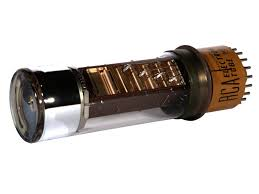
\includegraphics[scale=0.6]{figures/RCS/photomultiplier_tube}
\caption{A common photomultiplier tube \cite{PMT_picture}.}
\label{fig:PMT}
\end{center}
\end{figure}

The light sensing part of the PMT is the photo-cathode. This part is a negatively charged electrode coated with a photosensitive compound, located  the front of the tube and enveloped in vacuum. Due to the photoelectric effect, electron are emitted when a photon strikes the photocathode. Electrons emitted in the photocathode are picked up by an applied electric field and accelerated towards another electrode in the vacuum envelope, known as a dynode. The dynode works as an electron multiplier through secondary emission. When an electron generated in the photocathode strike the dynode, several new electrons are produced. These new electrons are then accelerated towards a secondary dynode where new electrons are subsequently emitted, thus further multiplying the electron amount. An anode then collects the electrons emitted by the dynodes, which provides a signal that can be read.

\begin{figure}[htb]
\begin{center}
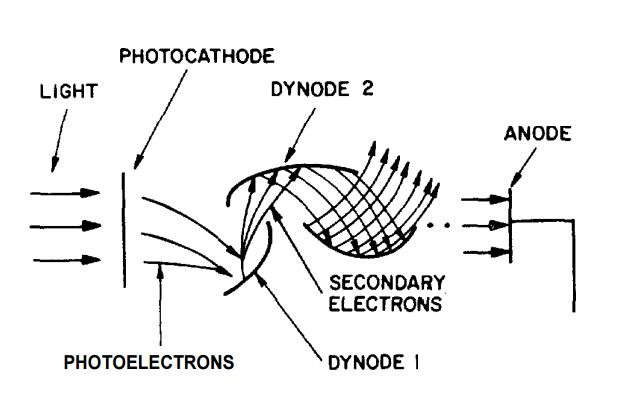
\includegraphics[scale=0.6]{figures/RCS/PMT}
\caption{An illustration of how the dynodes strengthen signal \cite{Dynode}.}
\label{fig:PMT_dynode}
\end{center}
\end{figure}

The strength of the PMT is the high gain this device is able to achieve with sufficient voltage. Gain is a term used to describe the amplification of a signal, which in the case of an optical sensor, is the ratio of the incoming photons to measured current output. In a PMT, each dynode increases the current as

\begin{equation}
    I_n = d_1 \cdot d_2 \cdot d_3 ... d_{n-1} \cdot d_n \cdot I_k
\end{equation}

Where $I_k$ is the photocathode current and $d_1 \rightarrow d_n$ are the dynode amplifications. A PMT tube is capable of reaching a gain of several tens of millions with enough dynodes and applied voltage as shown in figure \ref{fig:dynode_gain}

\begin{figure}[htb]
\begin{center}
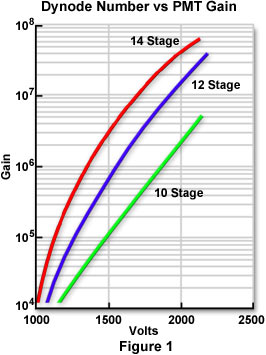
\includegraphics[scale=0.6]{figures/RCS/dynodegain}
\caption{A graph showing how the gain in a PMT increases with increased bias and increased number of dynodes \cite{Dynode_gain}.}
\label{fig:dynode_gain}
\end{center}
\end{figure}

Quantum efficiency is a measure for how many percent of the incoming photons that produce a signal in the photocathode. For PMTs, the quantum efficiency is around 30\% - 40\% depending on the type and the measured light spectrum, meaning that 60\% - 70\% of incoming photons are not detected. This is much lower than those of comparable light sensors such as APDs, with quantum efficiencies around 80\%.

The materials used for the photocathodes and windwos greatly influences the characteristics of the PMT. Most photocathodesare made of alkali metals from group 1 of periodic table known as alkali metals. Some of the common photocathodes are:

\begin{itemize}
\item Cs-I:\\
Caesium iodide is a type of ”solar blind” photocathode, meaning that it is not sensitive to solar radiation. Due to having low sensitivity at wavelenghts above 200 nm, this type of photocathode is used for ultraviolet radiation. 
\\
\item Cs-Te:\\
Caesium telluride is another type of solar blind photocathode. This type of photocathode is sensitive to wavelengths longer than 300 nm however.
\\
\item Cs-Sb:
Caesium antimony is sensitive in a much broader spectrum, capable of sensing both ultraviolet and visible light. Thus type of photocathode is favorable when when the intetnsity of the measured light is high.
\\
\item Bialkali (Sb-Rb-Cs, Sb-K-Cs:\\ 
Antimony-rubidium-caesium and antimony-potassium-caesium photocathodes are useful in both ultraviolet and visible spectrum. Compared to the caesium-antimony photocathode, the bialkali have higher sensitivity and lower dark current.
\\
\item Sb-Na-K:\\
antimony-sodium-potassium bialkali photocathode is sensitive in spectrum similar to the previous bialkali, but has lower sensitivity. This type of photocathode is able to withstand much higher temperatures, up to 175 $^circ$ Celcius, whereas other types of photocathodes usually go up to 50 degrees.
\\
\item Sb-Na-K-Cs:\\
The multialkali Antimony-sodium-potassium-caesium is useful from ultraviolet to near-infrared. This type of photocathode is also highly sensitive.
\\
\item Ag-O-Cs:\\ 
Silver-oxygen-caesium is sensitive from visible to near-infrared. This type of photocathode provides slightly lower sensivity in the visible region, but higher sensitivity in the high wavelengths compared to other photocathodes.
\\
\item GaAsP (Cs):\\
Caesium-activated Gallium arsenide phosphide photocathodes has higher quantum efficiency in the visible region. This is offset with no sensitivity in the ultraviolet region and high degradation-rate when exposed to high intensity radiation.
\\
\item GaAs (Cs):\\
Caesium-activated Gallium arsenide photocathodes provides sensitivity in a broad range, spanning from ultraviolet to near-infrared, with nearly flat, high sensitivity in most of this spectral range.
\\
\item InGaAs:\\ 
Indium gallium arsenide photocathodes are sensitive further into the infrared region than GaAs, while also providing good signal-to-noise ratio compared to other photocathodes useful in this region.
\end{itemize}

Due dark current, leakage current between dynodes, or high-energy radiation, PMTs can produce a signal in complete dark. Electronic noise which contributes to the dark current on top of thermally emitted electrons, is often included in the value of the dark current. The dark current is described as the small electric current that exists the device in the complete absence of photons. 

\subsection{Avalanche Photodiodes}
Avalanche photodiodes are a type of semiconductor-based, highly sensitive light detectors. Like PMTs, APDs convert radiation to electricity through the photoelectric effect, but operate using reverse voltage (voltage at the cathode is more positive than the voltage at the anode) rather than forward voltage. APDs exploit the avalanche multiplication in order to generate a readable signal, that is, radiation causes electrons to be excited in the detection material which is then accelerated by the applied electric field and excites more electrons. This process happen in the multiplication region of the device, which is made from a semiconducting material.

\begin{figure}[htb]
\begin{center}
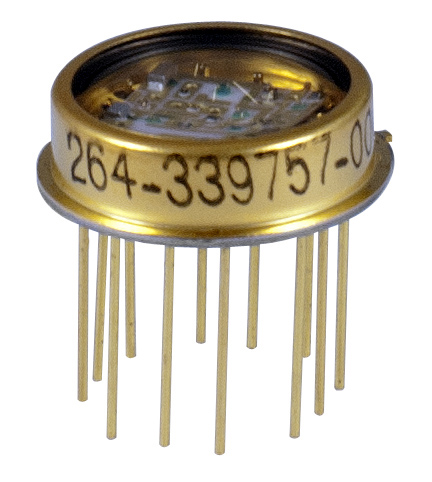
\includegraphics[scale=0.6]{figures/RCS/APD}
\caption{A common Avalanche photodiode \cite{APD_pic}.}
\label{fig:APD}
\end{center}
\end{figure}

The gain for APDs is much lower than what is attainable with PMT. At 100-200 volt reverse bias, typical gain values are around 100, and is strongly depend on the supplied voltage.  If the voltage is increased too much, breakdown will occur and the current in the diode will increase exponentially. A gain of this size is too small to detect single photons, but modern doping techniques have allowed for some avanlanche photodiodes to operate at applied voltage greater than 1500 volts allowing for gains up to 1000. This is not common APDs though, and these high gain APDs represent a small amount of highly modern APDs. These devices are much more sensitive in the near-infrared and visible regions compared to ultraviolet. APDs can reach quantum efficiencies of 80\% - 90\% at peak wavelengths, but as seen on figure \ref{fig:APD_specs}, the quantum efficiency drops sharply on either side of the peak.

\begin{figure}[htb]
\begin{center}
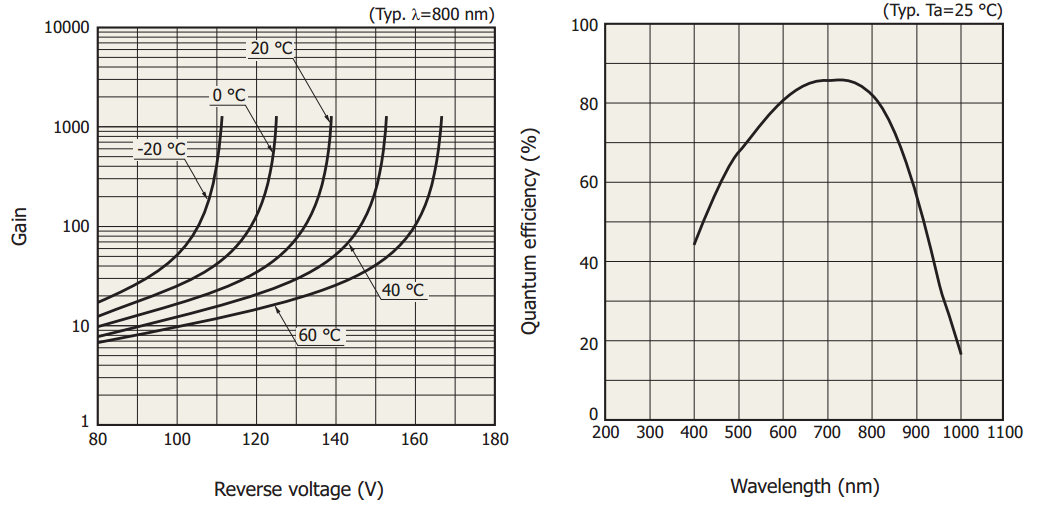
\includegraphics[scale=0.8]{figures/RCS/APD_specs}
\caption{Graphs of gain as function of temepature and bias for a highly sensitive, near-infrared, silicon APD (left). Quantum efficiency as function of wavelength for the same device (right) \cite{APD_graphs}.}
\label{fig:APD_specs}
\end{center}
\end{figure}

A way to measure single photons using an APD is activate Geiger mode, which is to operate it carefully just above breakdown voltage. In this state, even a single photon will produce a massive electron avalanche in the device which can then be read. During Geiger mode, the APD will need to rest between detections, lowering the detection frequency of the device. Thermally generated carriers within the device can also trigger avalanches, giving counts even in complete darkness.\\

APDs suffer from noise due to the nature of the electron avalanche process. This excess noise factor is denoted $F$, and for $k$ < 0.1 and $M$ > 20 can be approximated by the formula \cite{APD_noise}.

\begin{equation}
    F = 2 + k \cdot M
\end{equation}

where $k$ is carrier ionization ratio and $M$ is the gain of the photodiode. The square root of $F$ represents the factor by which the statistical noise of the APD rises above what would be expected from a noiseless multiplier due to only Poissonian statistics.\\

The  multiplication region of the APD is typically made of either silicon, germanium or Indium gallium arsenide.

\begin{itemize}

\item Si is sensitive in the visible and near-infrared area with low excess noise. Typical gain is 100, although it can be manufactured to attain up to 500. Excess noise factor is around 4.
\\
\item Ge is sensitive in the infrared region up to 1700 nm, but with high excess noise. Typical gain is 10 with excess noise factor of 9.
\\
\item InGaAs is sensitive in the infrared region. Typical gain is 10 and excess noise factor around 5.
\\
\item Gallium nitride can be used for an avalanche photodiode sensitive in the ultraviolet region. 

\end{itemize}

\subsection{The mission}

The purpose of the light sensor system is to search for light sources beneath the ice on Europa. It is interesting to search for light as the two main sources of light beneath the ice will either be from living organisms themselves in the form of bio-luminescence, or an energy source that life can potentially feed on. As such, if there is light beneath the ice, it is probable that any existing life will be close by. It must be expected that light sources will be difficult to find as it is likely that any source of light beneath the ice is both very rare and very weak. The water itself also has high absorption of light at certain wavelengths,as shown in figure \ref{fig:water_abs}, further increasing the difficulty of detecting light.  

\begin{figure}[htb]
\begin{center}
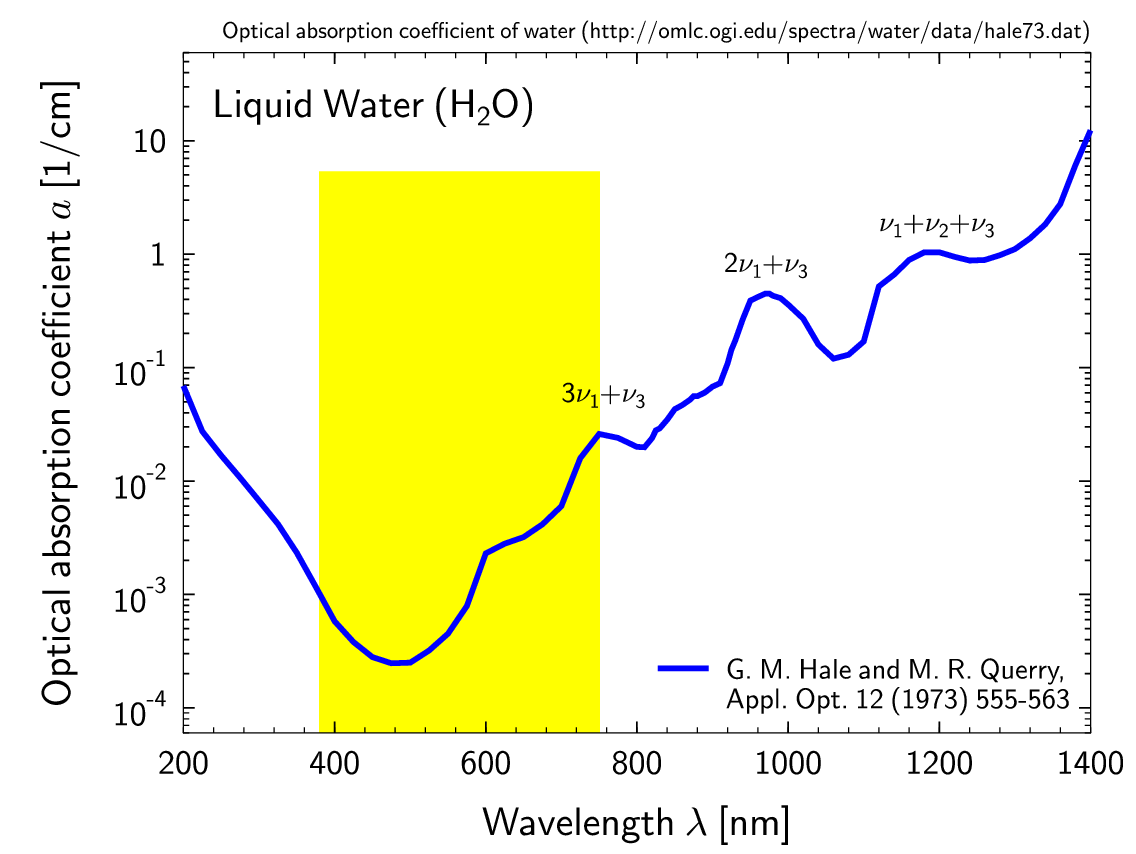
\includegraphics[scale=0.8]{figures/RCS/absorption_watef}
\caption{Graph of the absorption coefficient of water as function of wavelength \cite{water_abs}.}
\label{fig:water_abs}
\end{center}
\end{figure}

The light sensor system brought on the mission should therefore be as sensitive as possible in order to maximize the probability of detecting possible sources. Detection capability is not the only important parameter however, as weight and volume must be considered due to the limitations of space missions. Previously, two detection devices for light sensor systems has been discussed, the photomultiplier tube and the avalanche phototiode. The table below displays for each device some of parameters that are important to consider for choosing a light sensor system for the mission.\
	
%% table for PMT and APD parameters
\begin{center}
\begin{tabular}{ |c|c|c|c|c|c| } 
 \hline
               & QE & Gain & Mass & Size & Bias \\
 \textbf{PMT:} & 30\% - 40\% & Several million & 50-100 gram & Few centimeters & 1000-2000 V \\ 
 \textbf{APD:} & 80\% - 90\% & A few hundreds & A few grams  & Few mm or microns $\mathrm{\mu}m$ & 50-400 V \\
 \hline
\end{tabular}
\end{center}
	
The high gain of the PMT gives it an advantage over the APD in detecting weak sources. The higher quantum efficiency of the APD gives it an advantage in detecting rare signals as long as the signal is strong enough to warrant a response in the device. The essential difference is in the weight, size, and bias requirement, where the much smaller and lighter APD is more suited for space missions, as it is easier to integrate with the overall system. Despite its limitations in detection, the APD is favorable in every other aspect and is therefore the most suitable detection device for the mission.

\subsection{Bias power supply}
The APD will need a bias power supply to operate. For most APDs it will suffice to have 100-200 volt in reverse bias to attain maxium to gain without hitting the breakdown voltage, but up to 400 V can be needed for some specific high-gain APD. A bias power supply  further complicates the light sensor system as it increases the mass the and the volume significantly. The Hamamatsu APD module C5658 is a highly sensitive silicon APD build into a working module with a bias power supply, which will be used as baseline for the mass and volume requirements of and APD module \cite{APD_module}. 

\begin{figure}[htb]
\begin{center}
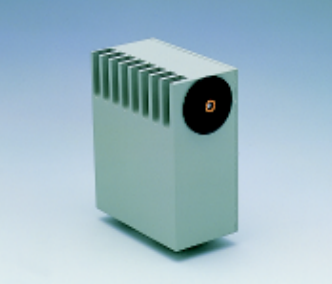
\includegraphics[scale=0.8]{figures/RCS/APDmodule}
\caption{The Hamamatsu APD module C5658 APD module \cite{APD_module}}
\label{fig:APD_module}
\end{center}
\end{figure}

This APD module weighs 120 g with a dimensional outline of 2.8 cm x 5.0 cm x 6.0 cm for a total volume of 84 $\mathrm{cm^3}$, making it both lightweight and small in size. With some optimization of the electronics, and by removing cover, it should be possible to get well below 80 g for the module. 

\subsection{Proposed models}
Two APD types are proposed for the Europa Life Finder Mission. The first model is for the visible spectrum of light, and the second is for the near-infrared spectrum.

\begin{description}
\item[Excelitas C30739ECERH]:
The Excelitas C30739ECERH Series APD is a high gain, large area silicon detector optimized for the visible spectrum. At 430 nm, the APD features 75\% quantum efficiency and can reach 450 gain. The chip spans an area of 6.5 mm x 6.5 mm and is operational at temperatures between 0$^circ$ and 50$^circ$ Celsius. The APD requires an operating voltage of 400 V in high gain mode. \cite{APD_visible}
\item[Excelitas C30921SH:]
The Excelitas C30921SH is a high gain near-infrared type silicon APD. This APD reaches 250 gain and the active diameter is 0.25 mm x 0.25 mm. \cite{APD_infrared}
\end{description}

The models are chosen specifically due to their high gain in order to minimize the weakness of the APD. The model chosen for the visible spectrum posseses the highest gain, but at the cost of high operating voltage. As the visible spectrum is where the water has the lowest absorption of light, having the best possible detection in this regime should be considered.

\subsection{Shielding}
The detection device will need to be shielded from the environment on Europa. As APDs function well at the low temperature in the environment, the shielding will focused on protecting the device from the water. Sufficient shielding can be made from simple metal tube sealed with a window at the front end made from suprasil, a quartz with high transparency in the ultraviolet, visible, and near-infrared regions. The structure of the tube will feature a light filtering lens between the window and the detector, and the electronic components furthest back.

\begin{figure}[htb]
\begin{center}
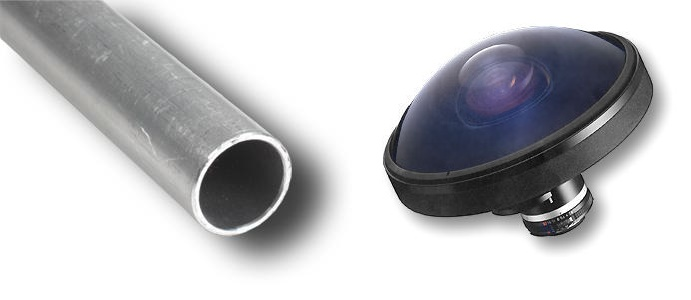
\includegraphics[scale=0.6]{figures/RCS/tube_fisheye}
\caption{An image of a simple aluminum tube as can be used to shield the sensor from water (left). An image of a common fisheye lens as will be used for window (right). \cite{Al_tube} \cite{Fisheye}}
\label{fig:tube}
\end{center}
\end{figure}

6061 aluminium alloy will be used for the tube, as it low density, and with adequate strength. On figure \ref{fig:wall_thick} is shown the tube wall thickness depending on tube radius at 100 bar pressure. It can be seen that with just a few millimeters of metal, the tube will be more than capable of withstanding the pressure beneath the ice on Europa.

\begin{figure}[htb]
\begin{center}
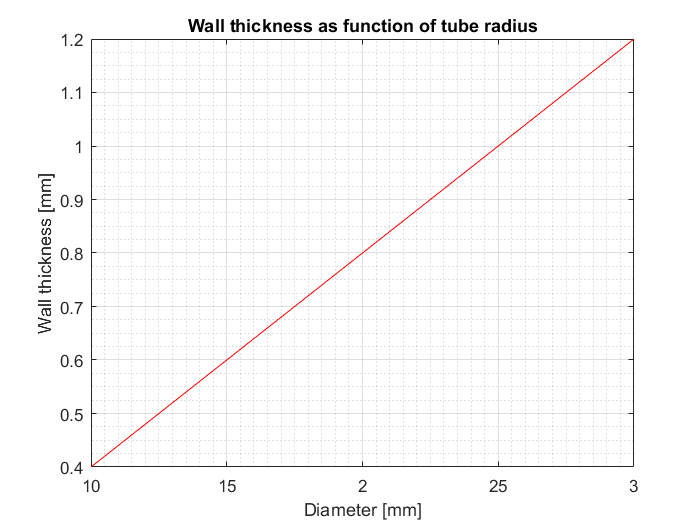
\includegraphics[scale=0.8]{figures/RCS/Wall_thickness_graph}
\caption{Graph showing the required wall thickness with increased radius of tube.}
\label{fig:wall_thick}
\end{center}
\end{figure}

The wall thickness is calculated from the stress in thin-walled cylinders. The equation is \cite{Wall_thickness}

\begin{equation}
    t = \frac{p \cdot r}{\sigma _c}
\end{equation}

where $t$ is the thickness of the wall, $p$ is the pressure and $\sigma _c$ is the hoop stress. As the yield strength of the aluminum alloy is 414 MPa, a maximum of 300 MPa stress was selected in order to ensure that the high strength of the metal ws utilized, but without causing any permanent to the tube. 

For avalanche photodiodes, the window will have to act as a focusing lens in order to increase the area of detection, and will therefore be designed as a fisheye lens. The window will sealed by placing an O-ring between the window and and tube edge and then bolting the window to the tube itself, a technique similar to that of high-pressure windows in submarines. A fisheye lens made of suprasil with a radius of 2 cm and a density of 2200 $\mathrm{kg/m^3}$ will weight in the area of 5 gram, with a half-sphere design. In total, it should be possible to construct an APD modul with shielding and focusing lens with mass and size as seen in table \ref{table:module}. 

%% table for APD module mass
\begin{center}
\label{table:module}
\begin{tabular}{|c|c|c|c|c|}
 \hline
               
 \textbf{Part:} & APD module & Aluminum tube & Lens & Total \\ 
 \textbf{Mass:} & 80 g & 7.8 g & 5 g & 92.8 g  \\ 
 \hline
\end{tabular}
\end{center}

\subsection{Conclusion}

This section has discussed possible light sensor systems for the Europa life-finding mission, and how to modify it for use in the environment beneath the ice on Europa. Between two different highly sensitive detection devices, photomultiplier tubes and avalanche photo diodes, the photo diodes were found to be the most suitable for a space mission due to low size, weight, and power consumption. The shielding used for the device is a thin aluminum tube sealed with a suprasil window, which is lightweight and more than able to withstand the pressure. A complete light sensor system unit with electrical components and shielding will be possible at less than 250 grams pr. sensor, making them light enough to be valid considerations for the mission. Due to how the quantum efficiency of APDs vary with wavelength of incoming radiation, it is suggested to use two units with different peak wavelengths such to ensure best possible detection in both the visible spectrum and the near-infrared spectrum. The ultraviolet spectrum can also be investigated, but as water has high absorption and APDs have low detection in spectrum, it will not be as efficient as looking in the visible and near-infrared.

\subsection{Further work}

The main discussion points that has been left out of the section are how many light sensor systems the mission should bring, and where to place them on the penetrator. Unlike many of the other life-finding devices, the light sensors will need to be placed so they have view of the outside through the window. This leaves many possible locations on the penetrator itself, but a more interesting set-up would be the robotic arm. Having the light sensor system placed on the arm would add mobility and the capability to search in a much wider area. Due to their light weight and size, it would be worth considering bringing several systems to look in several directions at once, vastly increasing the chances of detecting possible life. Further work in collaboration with the experts the robotic arm and mass budget experts would therefore be required in order to investigate whether these concepts would be possible. 

\autsection{Gas detector}{Agge Winther}

This chapter concentrates on why gas detection is important when searching for life, and how an instrument is designed for use in the penetrator to detect different gasses.

First a look into what gasses to be expected on Europa, next a look into gas detection under normal circumstances, and lastly a design of a gas detector for specific use in the ocean of Europa.

\subsection{Theory}

The main objective for this mission is to search for life. As explained in earlier chapters this could be found in many shapes and sizes. From bacteria to small living organisms, or perhaps alien life forms, unknown to science. If Europa is a life harbouring planet, and the ocean under the ice contains some sort of life. Then it would be an idea to also investigate extinct life.

Assuming the type of life can be compared to that of earth, we should be able to detect bi-products from living organisms. This chapter focuses on gasses, produced by living organisms, decomposed organic material or nutrients to support life.

As know from life and living organisms on earth, most life depend on the sun to create some sort of photosynthesis. Under the ice of Europa little to no light is expected to be found due to the thickness of the ice sheet above. Therefore traditional life, driven by the sun, is not to be found in the water of Europa, but for life harbouring conditions, some energy must be available.

Look back at earth, only a few places exist where life thrives, without light. One of them is around the black smokers on the ocean floor. The reason for mentioning this example is that Europa studies\cite{schmidtocean} show that a source of energy could be similar to the black smokers on earth. Life is found in great abundance around the smokers. First it was thought the organisms lived on marine snow, but the amount of life compared to the little amount of marine snow, would not be able to sustain the large amount of organisms found. Now it is know that the organisms thrive on the bacteria living around the smokers. This is called chemosynthetic bacteria, and instead of using photosynthesis the bacteria uses the nutrients and hydrothermal fluids from the smokers. The bacteria uses sulfur, methane and heat the create the energy need for life, this then feeds other life like clams and tubeworms, and usually a small ecosystem is found around black smokers, even if there is now sunlight. Some of the organisms around the smokers do depend on oxygen but anaerobic organisms are also found\cite{PMEL}.

This is good indication for life and even if the smokers are long gone, decomposition of the bacteria and ecosystems around the smokers could be seen in the levels of sulfur, methane, ethane, $CO_2$ and other hydrocarbons found in the water. Therefore sensors which can detect hydrocarbons would be ideal to bring with the penetrator down to the ocean, and look for these gasses.

\subsubsection{Searching for hydrocarbons}

Hydrocarbons are organic compounds made from carbon and hydrogen. Overall hydrocarbons can be dived in the 4 groups:
\begin{itemize}
  \item Saturated hydrocarbons (alkanes)
  \item Unsaturated hydrocarbons (alkenes)
  \item Cycloalkanes
  \item Aromatic Saturated hydrocarbons
\end{itemize}
Where methane and ethane is alkane's due to their single bond. On Earth most hydrocarbons come from decomposed organic matter, and it is this connection that will help conclude the kind of life on Europa.

Taking into account the smokers, organic material and simple life forms, simple hydrocarbons and other gasses would be found dissolve in the water or as gas bubbles. From this point on the focus shift towards detecting these gasses, which include: $SO_2$, H2S, $CH_4$, $NH_3$, $CO_2$, C2H6. The sensor need to be design must be able to detect as many as possible and if feasible, even bigger alkenes, alkanes and aromatic compounds.

\subsubsection{Detecting hydrocarbons at low pressure}

Detecting hydrocarbons can be done in many ways, first a look into how detection of gasses is done on Earth. This will give an idea on how today's methods could be modified and implemented in the instrument suite on the penetrator.

Most gas detectors are used to detect gasses harmful to humans, and leaks in pipelines. Most detectors are used to detect gasses in industry for safety reasons, helping to detect toxic, flammables or oxygen depletion, dangerous to workers or work safety. The most common ways to detect gas are:
\begin{itemize}
  \item Electrochemical
  \item Infrared
  \item Semiconductor sensor
  \item Ultrasonic
  \item Holographic
\end{itemize}
Electrochemical gas detectors diffuses the gas through a membrane, into an electrode, where it is oxidized. The reaction between the electrode and the gas generates an electric current which is linear to the gas concentration and by changing the membrane it is possible to custom design a detector for a specific gas. This type of sensor is very simple, stable and robust, but it is not perfect, it suffers from cross sensitivity and if it gets in contact with corrosive compounds, its life of operation is shortened\cite{intlsensor}.

Infrared gas detecting uses a whole other method to determining the gas in question. Here infrared light is passed through a known volume of gas, and the absorption of the different wavelength in the infrared spectrum is then analyzed. Different gasses have different absorption spectrums, like a fingerprint, and thereby the gas can be determined. This technique is more complex, but a lot more flexible compared to the electrochemical sensor, since it is able to detect different gasses with the same detector\cite{ndir}.

Semiconductor sensors detect gas by a chemical reaction with the semiconductor material, most used is tin-oxide, as gas comes in contact with the tin-oxide the resistance through the material drops. This type of sensor is commonly used for detection of methane, carbon monoxide, hydrogen, oxygen and alcohol-vapor.

Ultrasonic gas detectors are mostly used for detecting leaks, and cannot determine gas concentration. It works by listing for changes in the background noise around ultrasonic frequencies, since high pressure gas-leaks emit ultrasonic sounds, which can be detected. It is therefore no good for the type of detection wanted for this mission.

Lastly there are holographic gas sensors; they work under much the same principle as for the infrared detectors. Here the change in the reflected wavelength from the hologram can be used to determine the composition of the gas in front of the hologram. To work, they do require white light or lasers, which makes them more complex then the infrared sensors.

All of these methods mention above can be used on a gas, but a gas is just a state of the specific compound in question. On earth the gasses mentioned previously ($SO_2$, H2S, $CH_4$, $NH_3$, $CO_2$, C2H6) are naturally occurring as gas at sea level, (1 atm, 20 C), but this is not the case at the crushing pressure under the ice.

\subsubsection{Gas detection at Europas ice-sea surface}

The exact composition of Europas internal geology is still unknown. Qualified guess can be made dependant on pictures and its orbit. From this, it is estimated that the ice could be proximately 10km thick, all this ice generate an enormous pressure, estimated to be between 100-200bars at the ice-water barrier. Therefore what on Earth is a gas, would be a liquid or supercritical where the penetrator is sitting analyzing samples. To get a better insight into what happens to a compound mixed with water under this pressure a small study is done below.

At the ice-water barrier the temperature is around 273.15 Kelvin, below this the water starts to freeze and above it melts at a pressure of 100 bar\cite{PhaseH20}. At 200bar the temperature will be a 3 to 5 degrees Kelvin lower due to the pressure, but in general the freezing temperature is constant\footnote{This is for pure $H_2 O$}.

Overall a substance can have 3 states, gas, liquid or solid, it can also become super critical where it is in-between all 3 states. The way to characterize the states of a substance is through its phase diagram. An example of this is $CO_2$, which have the following phase diagram.

\begin{figure}[htb]
  \centering
  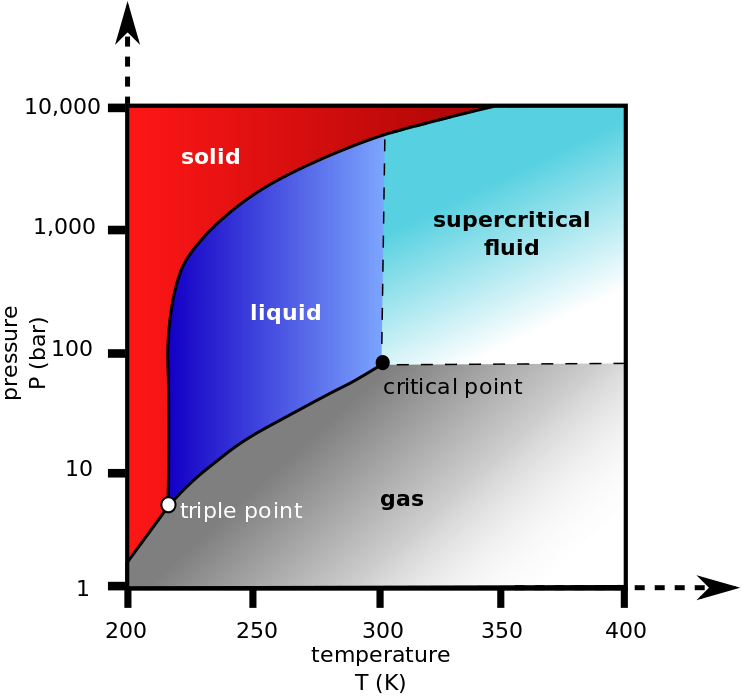
\includegraphics[scale=0.4]{figures/GasDetectionAgge/CO2PhaseDiagram}
  \caption{Phase diagram of $CO_2$, here the different phases are clearly seen, and how they depend on pressure and temperature\cite{PhaseCO2}}
  \label{fig:PhaseDiagramCO2}
\end{figure}

In the phase diagram of $CO_2$ (\ref{fig:PhaseDiagramCO2})it can be seen how the phases depend on pressure and temperature. If there is $CO_2$ present in the water at Europa, it would not be as a gas, because at 100 bar and 273.15 Kelvin $CO_2$ is liquid.

If $CO_2$ is present in the water, it is most likely to be mixed in the water, since water is a very good solvent for ionic and organic compounds, which makes most substances soluble in water; this is also the case for the gasses in question here. The solubility of substance in the water depends on the pressure above the solution. This follows Henry's law which states that the "solubility if a gas in liquid is directly proportional to the pressure above the surface of the solution\cite{SolubilityOfGases}".

This can be demonstrated with a bottle of soda. When the bottle is opened the pressure is released and CO2 starts to bubble up because the water cannot contain the same amount of $CO_2$ in the soda, under 1atm pressure.
As the phase diagram, a graph of the solubility of a substance can be made; here it is the solubility of $CO_2$ in water, but at atmospheric pressure:

\begin{figure}[htb]
  \centering
  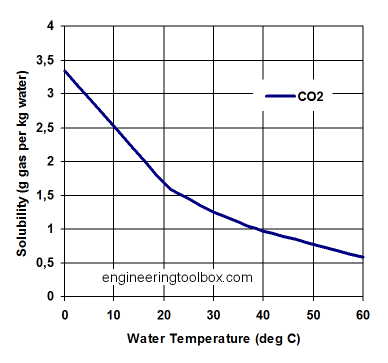
\includegraphics[scale=0.4]{figures/GasDetectionAgge/CO2Solubility}
  \caption{The solubility of $CO_2$ gas in water, at atmospheric pressure\cite{SolubilityOfGasesInWater}}
  \label{fig:SolubilityofCO2}
\end{figure}

From \ref{fig:SolubilityofCO2} it is seen that approximately 3.4 grams of $CO_2$ gas can solute in water at 273.15 Kelvin at a pressure of 1 atm. Combining this with Henry's law, the amount increases proportionally with the pressure, so the amount of $CO_2$ the water is able to solute is grater at 100 bar. Even when the $CO_2$ is liquid the solubility can be approximated as a gas/liquid solution\cite{SolubilityExplained}.

The conclusion on this is, it is not possible to use "normal" gas detecting methods, as discussed above. Other methods are needed to be able to detect what substances are present in the water. Some of the substances like $CO_2$ and $SO_2$ will be a liquid mixed with water, others might be a gas or super critical. The way of detecting the substances in the water needs to be done on another way.

\subsection{Implementation}

From the theory section it was discussed how to detect gasses, and what problems, and complications this have at high pressure, between the water and ice at Europa. The main problem in gas detection at Europa, concerned the fact that most of the gasses are liquid and not a gas. Therefore an instrument is design to take advantage of this high pressure condition. First the substances of interest are indexed according to their phase, solubility and at what pressure they change phase from liquid to gas (at constant temperature of 273.15 K) under the ice. Here the assumption is 100 bar and 273.15 degrees Kelvin.

\begin{table}
  \resizebox{\textwidth}{!}{%
  \begin{tabular}{|c | c | c | c|}
    \hline
     Substance: & Solubility: (g/kg water) & State: & Phase change pressure\cite{GasEncyclopedia} [Bar] \\ [0.5ex]
    \hline
    $SO_2$ (Sulfur dioxide) & 225 & Liquid & 1.5\\
    \hline
    $CO_2$ (carbon dioxide) & 3.4 & Liquid & 35\\
    \hline
    $NH_3$ (Ammonia) & 900 & Liquid & 4\\
    \hline
    $H_2 S$ (Hydrogen sulfide) & 7 & Liquid & 6\\
    \hline
    $C2H6$ (Ethane) & 0.13 & Liquid & 25\\
    \hline
    $CH_4$ (Methane) & 0.04 & Gas/Super & NA\\
    \hline
  \end{tabular}}
\end{table}

As mention in the Theory section, these substances are of great interest to detect possible life/extinct life in the water, for now on the focus will be on these 6 compounds for the further development of an instrument for the penetrator.

From the table above it is noted that all of the compounds are soluble in water, and most of them as a liquid at 100 bar and above. The notable characteristic is the phase change pressure, where the liquid changes phase to a gas. The important thing here is different pressures where the phase change happens, as for the IR-gas detector, this is a fingerprint tied to the compound. The odd one out is methane, it is still in a gas or supercritical state; it could therefore be detected with standard methods already known.  This will be investigated later.

The idea is to use an expansion chamber to boil of the gasses by lowering the pressure slowly. In constant temperature conditions a slow expansion of the gas, will give a characteristic pressure graph, with flat spots as the compound boils off and changes it phase. The principle can be seen in \ref{fig:PVdiagram} below.

\begin{figure}[htb]
  \centering
  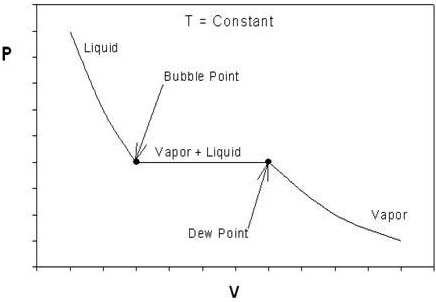
\includegraphics[scale=1]{figures/GasDetectionAgge/PVdiagram}
  \caption{PV-diagram with constant temperature. As the volume expands, the pressure drops, and the liquid changes state into gas}
  \label{fig:PVdiagram}
\end{figure}

In the PV-diagram, going from left to right, the liquid follows an isotherm as the pressure drops, when it reaches it phase change, and the liquid boils of into a gas. As this happens the pressure remains constant. With the help of a pressure sensor this can be detected, and the gas identified.

To create this phase change the pressure of the liquid under test needs to be dropped. If an expansion chamber is used then the Europa's liquid water will enter at a 100 bar or above, and then the pressure needs to be slowly drop down to 1 bar to detect compounds such as sulfur dioxide.

A traditional expansion chamber consists of a chamber with a moving piston that increase the volume in the chamber and thereby the pressure. This is not optimal for space exploration; firstly the need for moving parts is a source of unreliability and problems. Next to move the piston, a vacuum pump would be need. This also contains moving parts and is fragile, due to high pressure differences and high pressure seals, this method are therefore not ideal at all for the penetrator.

If it is not possible to create a low pressure by means on-board the penetrator, it needs to be brought from Earth, in small vacuum cylinders. This is a more reliable method but it life cycle is fixed to the number of cylinders brought with the penetrator.

\subsubsection{Detection chamber}

This method will consists of one chamber with the liquid sample under testing, and a vacuum cylinder connected through a small sealed hole into the test chamber. When the test chamber is ready for test the seal is punctured letting the pressure inside the test chamber slowly decrease, while the pressure is closely monitored. The pressure graph will then show the phase change of the compounds contained in the liquid under test. This method also shows other compounds than the 6 specified in the table above, this way if the predictions on what is contained in the water are wrong, the pressure graph will show it and it can afterwards be analyzed back on Earth. This is the design that will be used on the penetrator, the only down side to the instrument is it limited use, due to the vacuum cylinders. Take into account its simplicity, and that the water sample only takes place a few times due to the locked position of the penetrator, this is a good compromise.

\subsubsection{The mechanical design}

This subsection describes the overall mechanical design, including drawings and full description of functionality. First an overview of the complete system is presented:
\begin{itemize}
  \item Vacuum cylinder
  \item Test chamber
  \item Fill and empty mechanism
  \item Cylinder puncture
\end{itemize}
These are the 4 overall subcomponents and functions of the Vacuum Expansion Gas Analyzer (VEGA).

The vacuum cylinder, is based on the small canister, know from siphon bottle. In a siphon it is filled with $NO_2$ but could also contain a vacuum, in \ref{fig:Sipon} a picture of the cylinder is presented.

\begin{figure}[htb]
  \centering
  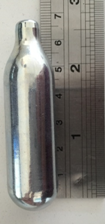
\includegraphics[scale=1]{figures/GasDetectionAgge/SiphonCylinder}
  \caption{A small gas cylinder from a Siphon. Instead gas, it would contain a vacuum}
  \label{fig:Sipon}
\end{figure}

A cylinder of this size has a volume of approximately 13 $cm^3$. This should be enough to let the gasses expand, since most of the liquid water on Europa is expected to be $H_2$O\footnote{\url{http://www.nasa.gov/topics/solarsystem/features/europa20130305.html}, 2016-05-07}, and therefore only a fraction of this is liquid gas. At the top of the cylinder, where it tapers in, the gas is released when punctured. This could be mechanized by a spring, loading the cylinder with nylon string and then burn the nylon string with a small electrode (copper wire) releasing the cylinder into a firing pin, with a small hole in to the test chamber slowly letting the liquid gasses expand.

The liquid under test is contained in the expansion/test chamber, where the vacuum cylinder is connected through the hollow firing pin. The chamber size compared to the vacuum cylinder is the most important ratio, since it determines how low the pressure in the test chamber becomes. The major fact is, as mention, how much liquid "gas" is contained in the water, in the theory section solubility was discussed, but here it was for a gaseousness substance mixed with water and not a liquid gas, further more the pressure is now much higher and Henry's law also needs to be taking into consideration. This part needs further investigation, but for now a good estimate of how much gas that would be in a water sample is 1 \%, this means that 99 \% of the sample is uncompressible. A chamber with a volume of 5 $cm^3$ would contain 0.05 $cm^3$ of liquid gas at 100 bar. To bring this down to 1 bar the volume needs to expand to 5 cm3, more than enough for a vacuum cylinder with a volume of 13 $cm^3$. This gives a satisfying pressure margin of more than 100 \%. Meaning that even with a pressure below the ice of 200 bar the chamber would still be able to reduce the pressure to less than 1 bar. Or if the liquid gas contained in the water is 2 \% of the total volume.

The test chamber needs to be filled and emptied after every use, with inlet and outlet ports in both ends of the chamber. Connected to the inlet and outlet will be a separate solenoid valve, and the pumping system from the other instruments will be utilized to circulate a water sample into the test chamber. The valve system will work by opening the inlet solenoid letting the water fill the chamber, then the valve closes, and the vacuum cylinder is released from its spring mechanism, slowly increasing the volume while the pressure is monitored. The chamber is now at around 1 bar pressure and the outlet valves opens equalizing the pressure, the inlet valve then opens and the chamber is flushed clean. It is very important to thoroughly flush the chamber to avoid any contaminants from previous samples, therefore it is suggested to let the inlet and outlet valve stay open and continually circulate the water surrounding the penetrator, through the chamber. This is of cause only if the sample is taken from the same place all the time, if the penetrator is able to pick up samples from other places then its surroundings a more complex flushing system needs to be implemented.

Lastly the puncture of the cylinder needs to be addressed, as already mention a spring loaded firing pin mechanism, would be the simplest way of implementing the vacuum puncture. This way no motors or valves would be needed, and therefore less points of failure. One of the main problems with this design is to close off the cylinder after the expansion has happened, to avoid that the test chamber volume increase. A way of avoiding this would be the use a two stage spring system, the first stage is fired and punctures the cylinder, when the expansion is done, the next spring fires and blocks the hole with the end of the firing pin.

\begin{figure}[htb]
  \centering
  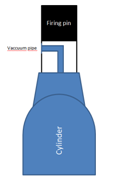
\includegraphics[scale=1]{figures/GasDetectionAgge/Firingpin}
  \caption{The black box is the firing pin where the first part contains the hollow part, which lets the expansion happen, and the solid black is the part that blocks the cylinder after use}
  \label{fig:FiringPin}
\end{figure}

In \ref{fig:FiringPin} an example of such a firing pin is sketched, the box with the black boarder is the firing pin, where the bottom part contains the hollow part, and the top part contains the seal of the cylinder after use. The first stage spring releases and punctures the cylinder, by sending the firing pin down to where the vacuum pipe exits, when the pressure is dropped the next spring releases sealing the cylinder.

The above 4 subsections explains the main parts of the VEGA-instrument, how it works and functions. From this, a hand drawing was made to show how it could look, and to get an idea of the overall dimensions and weight estimate. This first design was made to contain 6 cylinders in a rack structure:

\begin{figure}[htb]
  \centering
  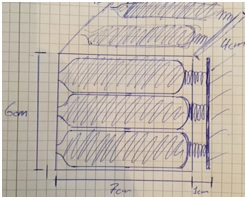
\includegraphics[scale=1]{figures/GasDetectionAgge/CylinderRack}
  \caption{A rack of 6 cylinders, with the spring in the back. Approximate dimensions are 6x8x4cm}
  \label{fig:RackOfSix}
\end{figure}

On \ref{fig:RackOfSix} a sketch of the structure for the cylinders can be seen, in the back the spring system is contained. This rack then connects to the chamber:

\begin{figure}[htb]
  \centering
  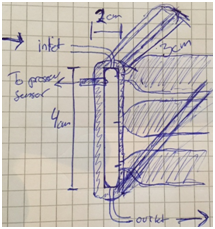
\includegraphics[scale=1]{figures/GasDetectionAgge/ChamberAndRack.png}
  \caption{Cross-section of the chamber and part of the vacuum cylinders, this chamber is 6 $cm^3$ and therefore a little bit too big}
  \label{fig:CrossSectionProto}
\end{figure}

In \ref{fig:CrossSectionProto} a cross section of the chamber is sketched, with part of the cylinder rack. As describe the liquid under test enter through the top inlet and exits at the bottom outlet (the valves are left out). Into the test chamber a pressure sensor is mounted to monitor the expansion. The firing pin is carved into the wall of the chamber and is not visible in the drawing, but when the cylinder is used, the spring will push the cylinder all the way into the wall of the chamber sealing it with the top of the firing pin.

\subsubsection{Principle prototype}

From the drawings and sketches a small prototype was made, which give an idea of how it would look if build. The prototype serves no practical function, and the firing pin or spring system is not build, this is just a chamber with in- and outlet and one cylinder attached.

\begin{figure}[htb]
  \centering
  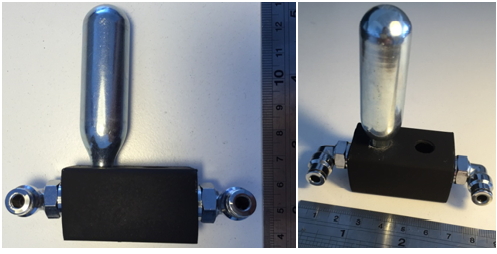
\includegraphics[scale=1]{figures/GasDetectionAgge/Prototype}
  \caption{A non working prototype of the VEGA-instrument. Here with only one cylinder added}
  \label{fig:NonProto}
\end{figure}

If the cylinders are mounted as showed in \ref{fig:NonProto} on the prototype it would be able to contain 7, since one port is used for the pressure sensor. It would be rater bulky due to the mounting of the cylinder on each side; therefore the rack system is more favorable. Overall it gives a good insight in the mechanical construction of the VEGA-instrument.

The last part not discussed is the pressure sensor, here it is possible to use an off the shelve part. Pressure sensors are today already used in harsh environments, and therefore only small modifications might be needed. A good example of a pressure sensor which is small compact and durable is the Festo SPTW-P100R-G14-VD-M12, which is a 0 to 100 bar sensor with a simple threaded connection, which simply screws into the chamber. It might be favorable with a sensor that has a range of 200 bar, but that is easily replaced if deemed necessary. A temperature sensor should also be mounted in the chamber to measure any temperature changes to make sure to get the optimal result.

With the VEGA-instrument not all the gasses specified earlier can be detected, one of the important ones is methane, but this is still a gas at the pressure between 100 and 200 bar, and can therefore not be detected with this expansion method. A way of detecting the methane would be to use a semiconductor sensor as mention in the theory section. This contains no moving parts, and is very simple to use and could be mounted inside the chamber, detecting methane when the chamber is flushed.

\subsubsection{Final physical specification}

When flying a space mission, mass, power consumption and volume of the instrument are very critical, they could be the difference flying the instrument or leaving it.

For the VEGA the configuration of it, inflects on the mass and volume, for this example the instrument carries 6 cylinders, and can therefore be reused 6 times. Dependent on the configuration of the cylinders and the camber the overall volume equates to approximately 200 $cm^3$ without the plumbing and wiring. The mass (build out of titanium) is 180 g for the cylinders, 150 g for the chamber, 120 g for sensor, 200 g for auxiliary. In all 650 g is needed for the whole instrument.

The power consumption for the instrument depends on what stage of use it is in. It does not require any power when not used. When in use the parts that use most power will be the solenoid valve for filling and emptying the chamber, which might draw a few watts when used. The gas sensor also uses a watt or less of power. In all peak consumption is assumed to be 5W, 1W when measuring, and no power use when standby.

There will also be some data processing and data transmission, but this is budgeted by the communication team. The instrument is not heavy on data, a measurement would contain between 5 and 10 Kbytes of data.

\subsection{Conclusion and further work on VEGA-instrument}

Through the design of the VEGA-instrument many different aspects has been covered, to make a comprehensive analysis of how such instrument should be designed for the harsh environment at Europa's ocean. Since this is only a theoretical instrument it is not sure that it will work at the conditions on Europa, therefore more work and test needs to be done. From the sections presented in this report, a prototype needs to be build and tests can begin, to see if it is possible to detect the gasses specified, and if other gasses also can be detected. Also an important aspect of testing is to see how large or small concentrations of a gas it is able to detect, this is dependent on the resolution of the pressure sensor and how much the gas expands when it is boiled of. The result will end up with a redesign of the instrument to accommodate the changes found under test.

Overall the instrument is a reinvention of a gas detector for high pressures, where conventional sensors are not able to work. The solution is simple and rethinks the way of sensing gas; the sensor is not perfect and is limited to a specific number of uses, due to the vacuum cylinders but this is a trade-off between complexity and simplicity. The same goes for the number of gasses it is able to detect, not all gasses can be detected but at the same time it will be able to detect more than compounds specified in this report. If the compound is liquid and mixed with the water, it could detect compounds not expected to be found and therefore the VEGA-instrument can extent it measurement range.


\autsection{X-Ray Flourescence Analyser}{Sebastian Helvig Christensen}

\subsection{X-ray fluorescence analyser}
Life on Europa requires an environment that can sustain it. To determine if the water under the ice of Europa can sustain life a chemical analyses of the water is needed. One such analyses is determining what elements are present in the water. For this purpose an X-ray fluorescence analyser is proposed.

\paragraph{Primary objective:}
To detect and quantify what elements are present in the water beneath the ice on Europa.


\subsection{XRF theory}

The X Ray Fluorescence (XRF) analyser irradiates a sample with x rays, and from the samples resulting fluorescence determines what elements are in the sample. 
When an atom is hit by a photon an electron can be knocked out of it’s orbit (primarily  the k shell), the following ‘replacement’ of this electron with an electron from a higher shell  will emit a photon which energy is characteristic for that element, this is called the characteristic x-rays or fluorescent x-rays. To knock an electron out of it’s orbit the incident photon have to be of a higher energy than the binding energy of the electron. The binding energy of electron in the k-shell increases with atomic number Z. 

\begin{figure}[htb]
	\centering
	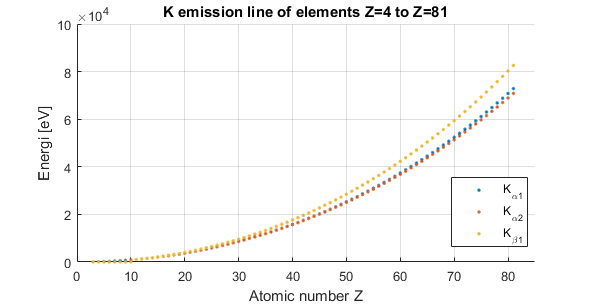
\includegraphics[width=\textwidth]{figures/XRF/Kalpha12Lines.png}
	\caption{$K_{\alpha 1}$, $K_{\alpha 2}$ and $K_{\beta 1}$ emission lines.}
	\label{fig:KalphaEmiLines}
\end{figure}

By measuring the energy of a sample's fluorescence photons, and the intensity at which they occur, the samples constituents and their quantity can be determined. Using this method elements as light as Beryllium (atomic number Z= 4) can be detected. The energy of the characteristic x-rays increase with atomic number, with very low energy x-rays for the light elements, 108eV for Beryllium (Z=4), to very high energies for heavier elements, 22keV for Ag (Z=47) and 71keV for Hg (Z=80).
The key components in an XRF analyser is the x-ray source and the x-ray detector. To increase performance x-ray optics can be added.

\subsubsection{X-ray source}
X-rays can be generated by bombarding a metal object with electron which have been accelerated through an electric field of up to several thousands volts. This is done in a vacuum tube called an x-ray tube, where a high voltage (100-80000V) is applied over a cathode and an anode. The electron are emitted from the cathode and when hitting the anode x-rays are emitted. If the electrons hit the anode with an energy higher than the anode atoms binding energy, they can knock inner electrons out of the orbit of the anodes atoms. The electrons which are knocked out from their orbit form the characteristic x-rays, this results in 'spikes' of high x-ray intensity around the anode metals characteristic x-rays line.
The electrons that do not interact directly with the atoms are slowed down in the anode metal and their energy is emitted as bremsstrahlung or braking radiation. The braking radiation form a continuous spectrum, with lower intensity for higher energies.
The intensity of an x-ray source is governed by the voltage applied and the intensity of te electron beam. The shape and direction of the beam is determined by the geometry of the anode, and the size of the electron beam spot on the anode.


\subsubsection{X-ray detector}
Measuring the fluorescent x-rays emitted can be done using two methods: Energy dispersive and wavelength dispersive. 
With the energy dispersive method the x-rays are directed towards a detector, where the x-ray photons induce a current proportional with. This process is repeated for every photon hitting the detector, creating a continuous stream of current pulses. These current pulses are recorded and sorted into discrete energy ranges by a Multi Channel Analyser (MCA). The result is a energy spectrum of the recorded x-ray photons. This method is suiteble for analysers who are designed to detect a range of elements, as it can detect a wide range of energies.
The wavelength dispersive method directs the fluorescent photons to a monochromator or diffractor before they are directed to a detector. The monochromator/diffractor ensures that only a narrow range (in terms of wavelength) of photons reach the detector. The detector used is commonly a photomultiplier which counts the incident photons. the result of an wavelength dispersive analysis is a measurement of the x-ray intensity at a specific wavelength. While multiple measurements can be done covering different wavelength, an energy dispersive method is better suited for this task.
For this mission the energy dispersive method is used.

\subsubsection{Mission specific criteria:}
Doing x-ray spectroscopy on Europa provides unique challenges that needs to be considere, when designing an instrument. The most prominent is:\\
\begin{itemize}
\item Operating at 130bar pressure.
\item Operating in a wet environment.
\item Analysing aqueous solutions.
\end{itemize}
These challenges will be discussed in the following sections.

\paragraph{High pressure environment}
Common XRF analysers consists of vacuum tube instruments, namely an  x-ray tube as X ray source, and the X ray detector. The interface between these instruments vacuum environment and the surrounding environment commonly consists of a thin (~0.1mm) Beryllium window. Beryllium is used because of it low X ray attenuation compared to its strength. When operating under the ice of Europa a vastly stronger window is needed, to be able to withstand the pressure.
Estimating the thickness of a clampedpressure window can be done with the following \citep{High_pressure_window}: 

\begin{equation}
\frac{F_a}{SF} = \frac{K \cdot D^2 \cdot P}{4 \cdot T^2} 
\end{equation}
\begin{equation}
\label{eq:PressureWinT}
T = D \cdot \sqrt{SF \cdot \frac{K}{4}} \cdot \sqrt{\frac{P}{F_a}}
\end{equation}

\noindent$F_a$ is the apparent elastic limit of the material [Pa].\\
SF: safety factor.\\
T: the thickness of the window [m].\\
K: empirical constant (1.125 for clamped windows with flexible fixture).\\
D: unsupported diameter of window [m].\\
P: pressure difference across window [Pa].\\

Using \ref{eq:PressureWinT} a 3mmØ beryllium window ($F_a$ at 240MPa \citep{BeMechanical}) with a safety factor of 8 results in a 1.05mm thick window. The Beryllium window will attenuate the fluorescent x-rays, and lower the detection limits.
Instead of a beryllium plate as a window, a polycapillary x-ray lens can be used. the polycapillary lens would function as the barrier between the vacuum environment and the high pressure environment, and focus/collimate the x-ray beam simultaneously. The polycapillary lens would need testing to make sure it can withstand the pressure. To seal off the end of the capillary tubes a beryllium film of 1-20um thickness could be used (assuming capillary diameter of 3-25um \citep{PolyCapOptics}, SF of 8 and $F_a$ at 240MPa).


\paragraph{Poly capillary optics}
Polycapillary lenses are a collection of thin tubes (capillaries), usually made from borosilicate glass, which direct x-rays through total external reflection. Total external reflection occurs when an incident photon enters the capillary and hits the glass wall at less than the critical angle. this is due to the differences in the refractive index of glass and the gas/vacuum of the capillary. This way any photon entering the tube at less than the critical angle is propagated through the capillary and its trajectory altered depending on the capillary curvature. Polycapillary lenses can be used for focusing or collimating purposes, by adjusting the curvature of the capillaries.
The focusing distance of a polycapillary lens is dependent on the photon energy and the focal spot size. It can be estimated using\citep{PolyCapOptics}:

\begin{equation}
FD = S \cdot \frac{E}{60}
\end{equation}

\noindent FD: focal distance [m].\\
S: spot size [m].\\
E: photon energy [eV].\\

The smallest focal spot commonly used is around 10um.
If used for focusing different energies the focusing distance will change. If used for focusing the fluorescent x-rays of a sample in the XRF analyser, a poly capillary lens will result in a focal ‘column’ of focal spots for the different energies. 


\paragraph{Wet environment}
As the environment is expected to be wet, it is necessary to consider the potential loss in the water. The sample is expected to be an aqueous solution, and there will be an attenuation of the X rays moving from the center of the sample outwards. 

The sample being an aqueous solution thus limits what we can detect further from the surface of the sample. The fluorescent X rays of the lighter elements (lower Z)  are lower in energy and will be attenuated more, as seen in \ref{fig:AttnH2O}.

\begin{figure}[h]
	\centering
	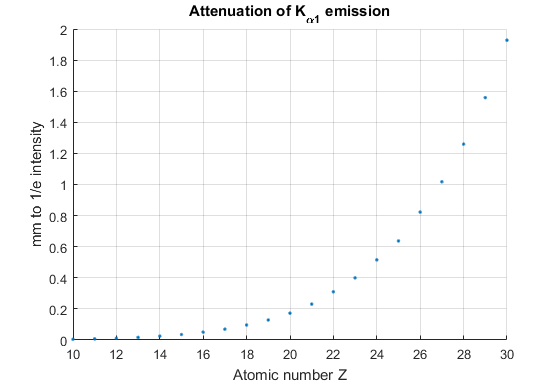
\includegraphics[width=0.8\textwidth]{figures/XRF/AttnOfKaplha.png}
	\caption{Attenuation of x-rays in H2O, in distance to 1/e intensity, for different elements\citep{XRay_Attn_H2O}}
	\label{fig:AttnH2O}
\end{figure}

% [INCLUDE PLOT OF WATER ATTENUATION OF X RAYS, AND WHERE THE ELEMENTS LIE IN THIS PLOT]  [Source http://henke.lbl.gov/optical_constants/ for attn & http://www.med.harvard.edu/jpnm/physics/refs/xrayemis.html for Kalpha line]

Detecting elements in the lower region, lighter than Cobalt (Z=27, $K_{\alpha 1}$ at 6.9keV), could prove difficult through more than 1 mm of water, due to the fluorescent photons being attenuated very heavily. 


\paragraph{Compton scattering in water}
When subjecting an aqueous sample to X ray irradiation, Compton scattering have to be taken into account. The Compton scattering results in reflected X ray photons depending on the incident photons energy, and the reflected angle. Energy of the scattered photons can be estimated with \ref{eq:ComtonEQ} \citep{ComptonScatt}:

\begin{equation}
\label{eq:ComtonEQ}
hv' =  \frac{hv}{ 1+alpha*(1-cos(theta)) }
\end{equation}

\noindent hv': energy of the reflected photon.\\
hv: energy of the incident photon.\\
alpha: $\frac{hv}{electron rest energy (0.511MeV)}$ \\
 
The scattered photons are scattered evenly in all directions. Thus the scattering results in a distorted mirror of the incident photon energy spectrum. If the incident spectrum is concentrated in a narrow energy band, it can mask some fluorescent x-rays in the sample.

%If an x-ray source of 17.5 keV is used, the resulting compton peak will be in the range of 16.3keV to 17.5keV. This will intersect with the Kalpha line of Yttrium (Z: 39) and Zirconium (Z: 40), and possible further depending the consistency, in terms of photon energy, of the x-ray source. It is thus important to pick an x-ray source that will not obscure important elements with the compton scattered radiation.




\subsection{XRF Implementation}

\subsubsection{X-ray source}
To incite fluorescence in heavy elements, a high energetic source is needed, as high energy photons is needed to knock their electron out of their orbit. To achieve this a x-ray tube with an Ag anode with an output spectrum as seen in figure \ref{fig:AgSpectra} is recommended. The high energy of the peaks enable the source to achieve fluorescence from elements up to Ag (Z=47), with lesser efficiency up to Sm (Z=62, 40keV).

\begin{figure}[h]
	\centering
	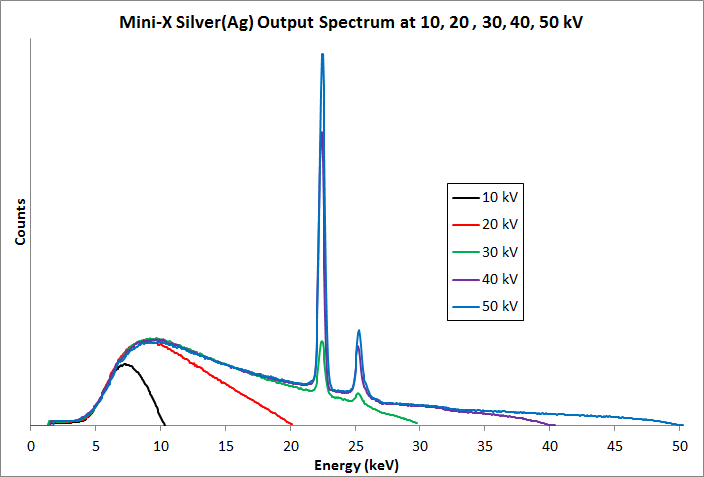
\includegraphics[width=\textwidth]{figures/XRF/minix50_ag6.png}
	\caption{Output spectrum for a x-ray tube using an Ag anode at different voltages.\citep{AmptekSource}}
	\label{fig:AgSpectra}
\end{figure}

The lower end of the energy spectrum is caused by bremsstrahlung in the anode, and is not of much use as it provides little additional resulting fluorescence. The low end is also scattered and will provide a significant noise source for the lower energies. This is particularly undesirable as the lighter elements low energy fluorescence, are also heavily attenuated by the water they are dissolved in. To adjust the spectrum an Al filter can be used to attenuate the lower energies, as seen in figure \ref{fig:AgSpectraFilt}.

\begin{figure}[h]
	\centering
	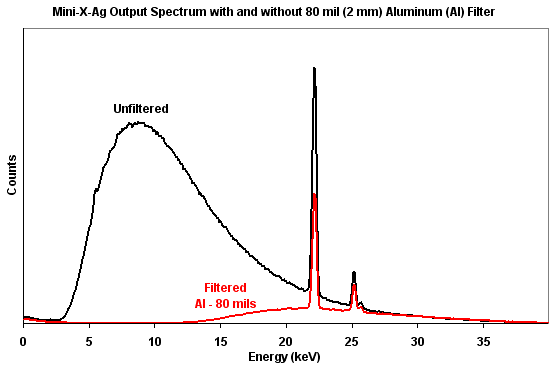
\includegraphics[width=\textwidth]{figures/XRF/minix_Fil.png}
	\caption{Filtered and unfiltered Ag x-ray tube spectrum at 40keV. \citep{AmptekSource}}
	\label{fig:AgSpectraFilt}
\end{figure}


The output spectrum of the x-ray tube have to significant peaks at ~23keV and ~25keV. This is the characteristic lines of Ag when subjected to electron radiation. Knowing these line enables us to take them into account as they will show up as noise in measurements. Focusing on the remaining peaks, and using equation \ref{eq:ComtonEQ}, the Compton scattering resulting from the incident spectrum can be estimated in figure \ref{fig:AgSpectraCompton}.

\begin{figure}[h]
	\centering
	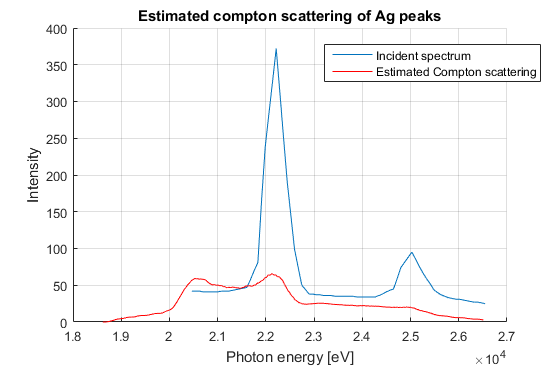
\includegraphics[width=\textwidth]{figures/XRF/estComptonAgPeaks.png}
	\caption{Estimated Compton scattering of the source spectrum.}
	\label{fig:AgSpectraCompton}
\end{figure}

The resulting noise peaks from Compton scattering lies between 20keV and 22.5keV. These will overlap with the $K_\alpha$ of Pd (Z=46, $K_\alpha$ at 21.1keV) and Ag (Z=47, $K_\alpha$ at 22.1keV).

\paragraph{Instrument}
Creating the high voltage needed for the instrument a voltage tripler can be used. The entire instrument can be realized (including high voltage powersupply) with\citep{AmptekSource}:\\
Mass: 360g\\
power: 9W (at max output intensity)\\
Volume: 272.24cm3

\subsubsection{X-ray detector}
When considering the detector the range of encountered photons should be considered. The lighter elements $K_\alpha$ lines are only a few hundred keV apart, to differentiate these a suitable resolution is needed. Detectors also do not perform equally across all energies. The lower limit of the detector is determined by the detector window, as low energy photons are quickly attenuated. The higher limit is determined by the detector material. If we used a polycapillary lens, a window of 25um Be can be used. The detector material can be chosen as Si, as it provides a greater range than what we expect to achieve fluorescence from. In figure \ref{fig:AmptekDetector} a plot of differing detector can be observed. The resolution of the 25um Be SI-PIN detector is sufficient to distinguish elements heavier than Na.

\begin{figure}[h]
	\centering
	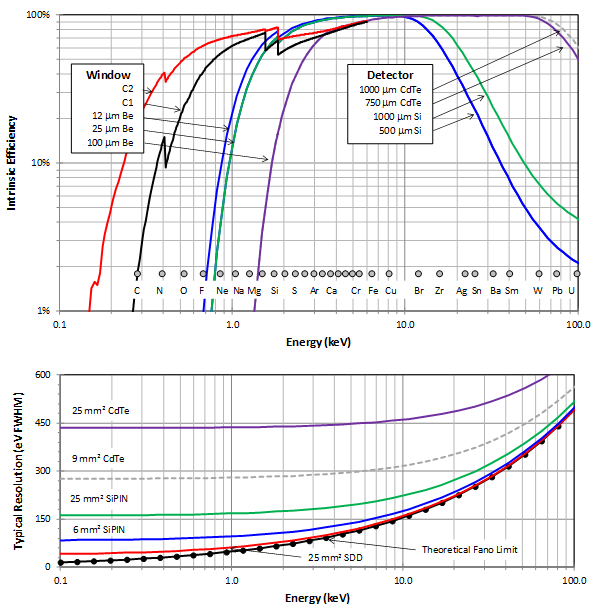
\includegraphics[width=\textwidth]{figures/XRF/EnergyRes.png}
	\caption{\cite{AmptekDetector}}
	\label{fig:AmptekDetector}
\end{figure}





\paragraph{Instrument}
The entire instrument, including high voltage power supply and MCA, can be realized with\citep{AmptekDetector}:\\
Mass: 180g\\
power: 4W max, 2.5W typical\\
Volume: 175cm3



\subsubsection{Mass, power and volume}






\autsection{HPLC}{Morten Lykke Hilligsøe}
\label{sec:hplc}
High-performance liquid chromatography (HPLC and also known as high-pressure liquid chromatography), is a chemical technique commonly used to identify, quantify and separate components of a liquid sample. Most commonly, the technique uses pressure to pump a solvent through a column filled with silica beads covered in carbohydrates. The silica beads typically have a size range of 2–50 micrometers in diameter. By mixing the sample with a polar solvent, such as acetonitrile or methanol, and passing it through the highly non-polar silica beads, each component of the sample will interact differently with the column, thereby affecting flow rates of each compound and making it possible to separate them. \cite{wiki_hplc}

Many different HPLC techniques exist, including:
\begin{itemize}
    \item Partition chromatography
    \item Normal–phase chromatography
    \item Displacement chromatography
    \item Reversed-phase chromatography (RPC)
    \item Size-exclusion chromatography
    \item Ion-exchange chromatography
    \item Bioaffinity chromatography
    \item Aqueous normal-phase chromatography
\end{itemize}
with reversed-phase chromatography equipment being very common in chemistry and biochemistry labs all over the world. In reversed-phase chromatography, the components of the sample mixture are separated from each other based on their different interactions with the absorbent particles of the HPLC column, also known as the stationary phase. The pressurized sample/solvent mixture is referred to as a "mobile phase".

\subsubsection{Detection}
HPLC can detect a vast array of different chemical and biochemical compounds, including many compounds considered direct indicators of present life \cite{hplcbasics}:
\begin{itemize}
    \item DNA and RNA
    \item Pharmaceuticals like aspirin, ibuprofen, or acetaminophen (Tylenol) 
    \item Salts like sodium chloride and potassium phosphate 
    \item Proteins like egg white or blood protein 
    \item Organic chemicals like polymers (e.g. polystyrene, polyethylene) 
    \item Heavy hydrocarbons like asphalt or motor oil 
    \item Many natural products such as ginseng, herbal medicines, plant extracts 
    \item Thermally unstable compounds such as trinitrotoluene (TNT) and enzymes 
\end{itemize}
HPLC will not be able detect all of these compounds using a single HPLC column, as different types of columns are optimized for different detection schemes, but a single column will still be able to detect a vast range of compounds. If more compounds are to be detected, a setup with multiple columns could also be designed. Special HPLC setups can also separate and quantify chiral enantiomers, which are considered clear indicators of life, if a set of enantiomers are found in varying concentrations. Such setups are however much less versatile, and are better suited for experiments where the examined compound is known beforehand.
Typically a marker solution is introduced to the system before the sample, in order to have some reference points. Detection limits depends very much on the optical setup (light source \& sensor) and the compound to be detected, but the separation of compounds reduces noise, thereby making it possible to detect concentrations down to µg/L, with just a few µL of sample. Because of these small sample amounts, typical column dimensions are just 2.1–4.6 mm in diameter, and 30–250 mm in length.

\begin{figure}[htb]
	\centering
	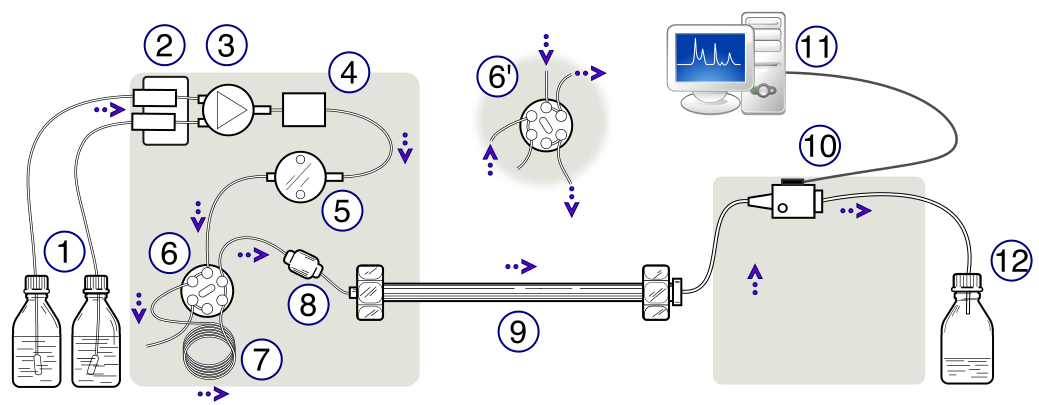
\includegraphics[width=\textwidth]{figures/mlh/HPLC.png}
	\caption{Schematic representation of an HPLC unit. (1) Solvent reservoirs, (2) Solvent degasser, (3) Gradient valve, (4) Mixing vessel for delivery of the mobile phase, (5) High-pressure pump, (6) Switching valve in "inject position", (6') Switching valve in "load position", (7) Sample injection loop, (8) Pre-column (guard column), (9) Analytical column, (10) Detector (i.e. IR, UV), (11) Data acquisition, (12) Waste or fraction collector.\cite{wiki_hplc}}
	\label{fig:HPLC}
\end{figure}

\subsubsection{Components}
Figure \ref{fig:HPLC} illustrates a typical HPLC system. 5 major components are required for a HPLC setup:
\begin{enumerate}
    \item Pump: The pump is used to force the sample/solution mixture through the column at high pressure and at a specific flow rate. HPLC flow rates are commonly in the 0.1- to 8-mL/min range, with a pressure gradient commonly in the range of 50- to 600-bar.
    \item Injector: The injector introduces the sample into the solvent (mobile phase) flow stream at typical volumes of 5- to 20-µL. As the sample is unpressurized, the injector must be able to withstand the high pressure of the system.
    \item Column: The column’s stationary phase separates the sample components of interest using various physical and chemical parameters, such as polarity, porosity or bioaffinity. The small particles that make up the inside of the column is what causes the high pressure gradient at normal flow rates. 
    \item Detector: The detector can detect the individual compounds in the column output (elute). Usually a UV or wide spectrum light source is used in combination with a sensor which can detect individual wavelengths (e.g. photodiode array). By detecting the individual wavelength absorption of the elute, components can be distinguished, identified and quantified. The elute absorption as a function of time, is the liquid chromatogram result.
    \item Computer: Finally, a computer is used to control the HPLC instruments and might also be used to analyze the resulting chromatogram. As a result, the resulting data of each experiment can vary from megabytes when high resolution chromatographs are transferred, over kilobytes when low resolution chromatographs are transferred, and all the way down to single bytes for yes/no answers or concentrations at specific retention times. 
\end{enumerate}

Besides these components, a HPLC system usually also includes a solvent mixer and a degassing system. 
The mixer is used to create the desired mobile-phase composition, typically from a mix of water, acetonitrile and/or methanol. The mixer isn’t strictly necessary, as one can use a premade mobile-phase solution, but often a gradient of these compounds are desired throughout the experiment, as the mobility range of different compounds would otherwise be too vast, e.g. some move directly through the column, and others doesn’t move at all.

The degassing system is an essential part of any HPLC system used under normal lab conditions, as it ensures that no bubbles are created when the mobile-phase traverses the negative pressure gradient of the HPLC column. Such bubbles will ruin the experiment by blocking any further movement through the column, and can even potentially break the column.  Commonly used degassing practices for HPLC mobile phase are helium purging (removes up to 80\% of all gasses), vacuum degassing (up to 60\%) and sonication (up to 30\%). However, degassing would not be a problem on a subsea space mission for two reasons: 
\begin{enumerate}
    \item The system is closed and all solvents can easily be degassed before departure.
    \item The experiments are performed under high-pressure external conditions (below several kilometers of ice), making sure that the pressure never drops low enough for bubbles to occur.
\end{enumerate}

\subsubsection{Implementation}
To implement a HPLC system on the Europa subsea mission, the system will have to be limited in the power usage, weight, volume, and data transfer rates. The following equipment has been used as reference for calculating an approximate weight, power and volume usage:
\begin{itemize}
    \item 0.01-10mls/min, 143bar, Stainless Steel, positive displacement piston pump \cite{hplc_motor}
    \begin{itemize}
        \item Weight: 1.6kg
        \item Power: 40.8W
        \item Size: 139.7mm x 76.2mm x 266.7mm
    \end{itemize}
    \item Injector \cite{hplc_injector}
    \begin{itemize}
        \item Weight: 0.25kg
    \end{itemize}
    \item C18 Reversed-Phase HPLC Column \cite{hplc_columns}
    \begin{itemize}
        \item Weight: 0.2kg
        \item Size: 200mm x 2.2mm (internal)
    \end{itemize}
    \item 190-500nm, 13nm resolution, UV Detector \cite{hplc_detector}
    \begin{itemize}
        \item Weight: 1.5kg
        \item Power: 60W
        \item Size: 121mm x 129mm x 187mm
    \end{itemize}
    \item Solvent
    \begin{itemize}
        \item 50ml per experiment
    \end{itemize}
\end{itemize}
The chosen pump is a displacement piston pump, which are commonly used high pressure low volume applications such as HPLC systems. The possibility of using a peristaltic pump was also examined, but no peristaltic pumps were found, which could operate at +100bars of pressure. Both the injector and HPLC column weights are estimates, as no weights were given by the manufacturers. It would be nice to include a UV-Visible detector which isn’t limited to 500nm detection range, but this component was the most weight efficient solution available. Finally the solvent volume is calculated as:
\begin{equation}
    1ml/min \cdot 30min = 30ml    
\end{equation}
Which is then rounded up to 50ml per experiment, because some solvent is also necessary to flush the column before experiments.

Several connectors and peripheral equipment will also be required, resulting in a system which, during operation, requires a power input of approximately 100W, and has a total weight of around 4kg plus approximately 0.05kg of solvent per experiment. The volume and mass of the individual components are quite large when considering the size of the penetrator, but by stripping each component down to the bare minimum, e.g. getting rid of shielding, user interfaces and AC-DC converters, the size and weight should be low enough for the HPLC solution to be contained within the penetrator. 

The data transfer rates can be calculated from the sampling frequency $f$, the sampling range $l$, the sampling resolution $\delta$, and the bit-size $b$ of each measurement point:
\begin{equation}
    f \cdot \frac{l}{\Delta} \cdot b = 1Hz \cdot \frac{500nm-190nm}{13nm} \cdot 12bits = 286bps
\end{equation}
Here the sampling frequency is chosen to be 1Hz, which is on the low end of standard sampling rates of laboratory HPLC experiments, but still good enough for most experiments. The 12 bit measurement point size gives a range from 0-4095. Since the HPLC isn’t expected to run continuously, but only run when an interesting sample has been up-concentrated, the 286bps is far below the maximum transfer limit, and both sampling frequency, sample points and bit size may be increased without creating a bottleneck.

A simple illustration of the system is presented in figure \ref{fig:hplc_drawing}.
\begin{figure}[htb]
	\centering
	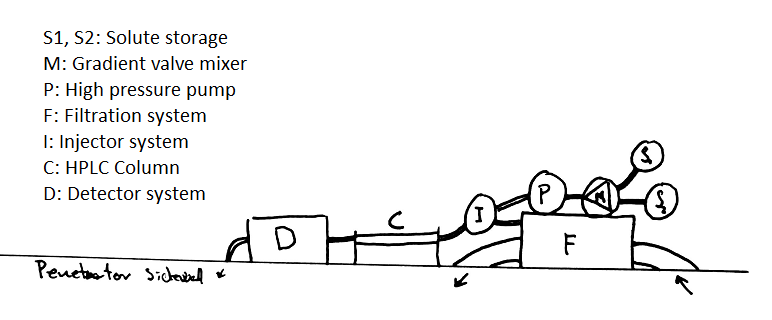
\includegraphics[width=\textwidth]{figures/mlh/HPLC_system}
	\caption{}
	\label{fig:hplc_drawing}
\end{figure}

\autsection{Lab-on-a-chip \& microscopic sensors}{Morten Lykke Hilligsøe}
Lab-on-a-chip (LOC) systems are a common description of microfluidic devices which can perform one or several laboratory functions on a single chip. Lab-on-a-chip systems are often characterized by a very small size in the mm2 – cm2 range, high automation requiring only sample injection and result identification, as well as zero chance of contamination due to the closed system. The small size of LOCs also results in extremely small sample sizes, sometimes reaching less than a pico liter, which can be both an advantage and a disadvantage, as small amounts of the compound of interest is necessary for detection or analysis, but the small sample volumes can be hard to handle properly. \cite{wiki_loc} \cite{labchip}

LOCs are typically constructed using the same lithographic techniques developed by semi-conductor industry for integrated circuit production, and consists of µm or sub-µm sized mechanical structures such as channels, mixers, valves, pumps and dosing devices, combined with micro-sensors, chemical \& biochemical reagents and/or external sensors, e.g. optical or electrical sensors. LOCs are still a novel technology, but the technology is quickly evolving and LOC solutions have found many uses, especially within biochemical and microbiological analysis, such as bacteria, virus, and bioanalyte detection. \\
\cite{Ghallab2004} \cite{Pawell2013} \cite{Pawell2015} lists advantages and disadvantages of LOCs as:

Advantages of LOCs:
\begin{itemize}
    \item low fluid volumes consumption (less waste, lower reagents costs and less required sample volumes for diagnostics)
    \item faster analysis and response times due to short diffusion distances, fast heating, high surface to volume ratios, small heat capacities.
    \item better process control because of a faster response of the system (e.g. thermal control for exothermic chemical reactions)
    \item compactness of the systems due to integration of much functionality and small volumes
    \item massive parallelization due to compactness, which allows high-throughput analysis
    \item lower fabrication costs, allowing cost-effective disposable chips, fabricated in mass production
    \item part quality may be verified automatically
    \item safer platform for chemical, radioactive or biological studies because of integration of functionality, smaller fluid volumes and stored energies
\end{itemize}
Further advantages for use on space missions, includes the possibility for complete sample processing in a single chip, e.g. filtration, lysing, mixing, chemical reactions and positioning, thereby reducing or completely dismissing any requirements for large and bulky laboratory equipment typically necessary to prepare samples before any analyte can be detected.

Disadvantages of LOCs:
\begin{itemize}
    \item novel technology and therefore not yet fully developed
    \item physical and chemical effects—like capillary forces, surface roughness, chemical interactions of construction materials on reaction processes—become more dominant on small-scale. This can sometimes make processes in LOCs more complex than in conventional lab equipment
    \item detection principles may not always scale down in a positive way, leading to low signal-to-noise ratios
    \item although the absolute geometric accuracies and precision in microfabrication are high, they are often rather poor in a relative way, compared to precision engineering for instance.
\end{itemize}
Further disadvantages for use on space missions, includes that many LOCs are single-use constructions, thereby requiring extra storage space if the experiment is to be performed multiple times, as well as mechanics to switch between chips. Then novelty of LOC technology is also exemplified in the fact, that even though the chip itself can be very small, the external equipment necessary to operate the chip is often standard laboratory equipment which hasn’t been scaled accordingly.

\subsubsection{Systems of interest}
Below is described 4 systems of interest for a life detection mission. Many other relevant projects exists, ranging from small research projects to a few readily available solutions.

\paragraph{DNA extraction and real-time PCR \cite{Oblath2013}}
In an article from 2013, researchers at the University of North Carolina describe a “microfluidic chip integrating DNA extraction, amplification, and detection for the identification of bacteria in saliva”. Such a device could easily be used to detect if DNA is present on Europa. And because the chip has integrated filters, minimal preparation of the sample is required. The system works by filtering lysed organisms through a nanoporous aluminum oxide membrane, followed by PCR amplification of the filtered DNA in 7 parallel reaction wells. PCR amplification is the standard method of up concentrating DNA, and using this method the chip was able to detect as low as 8-12 copies of methicillin-susceptible Staphylococcus aureus DNA. PCR amplification depend primers to attach to matching DNA sequencing. For a Europa mission, any microorganisms will of course be unknown, and specific target primers will not be available. Instead a series of general primers which bind to DNA sequences common to earth life can be used to simply detect DNA. 
\begin{figure}[htb]
	\centering
	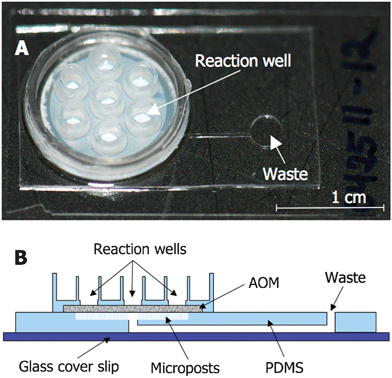
\includegraphics[width=\textwidth]{figures/mlh/reactionwells.png}
	\caption{Image of a DNA extraction and real-time PCR chip (A) and a schematic of its cross-section (B). Schematic is not to scale. The glass cover slip is 150 $\mu m$ thick, the microfluidic base of the chip is \~400 $\mu m$ thick, The AOM is 60 $\mu m$ thick, and the reaction wells are \~2.8 mm tall. The microposts are 75 $\mu m$ in diameter and 18 $\mu m$ tall. The microfluidic channel is 30 $\mu m$ deep and 1.6 cm long. \cite{Oblath2013}}
	\label{fig:DNAPCRchip}
\end{figure}

\paragraph{Chemical sensor \cite{Schwarz2014}}
Although more a sensor than LOC, in 2014, researchers at Vienna University of Technology have developed a very interesting sensor chip, for measuring the chemical composition of liquids. The sensor works by placing a matching set of mid-infrared quantum cascade laser and detector on a single chip connected through a 50 $\mu m$ waveguide. When specific molecules pass close to the waveguide, the laser light is absorbed and the molecule can be detected. The wavelength of quantum cascade lasers can be finely tuned, and lasers matching specific molecules can therefore be created, allowing for detection of various molecules, such as carbohydrates or proteins, and the small size will make it possible to have a whole array of various wavelength sensors to measure the concentration of many different compounds using a single chip.
\begin{figure}[htb]
	\centering
	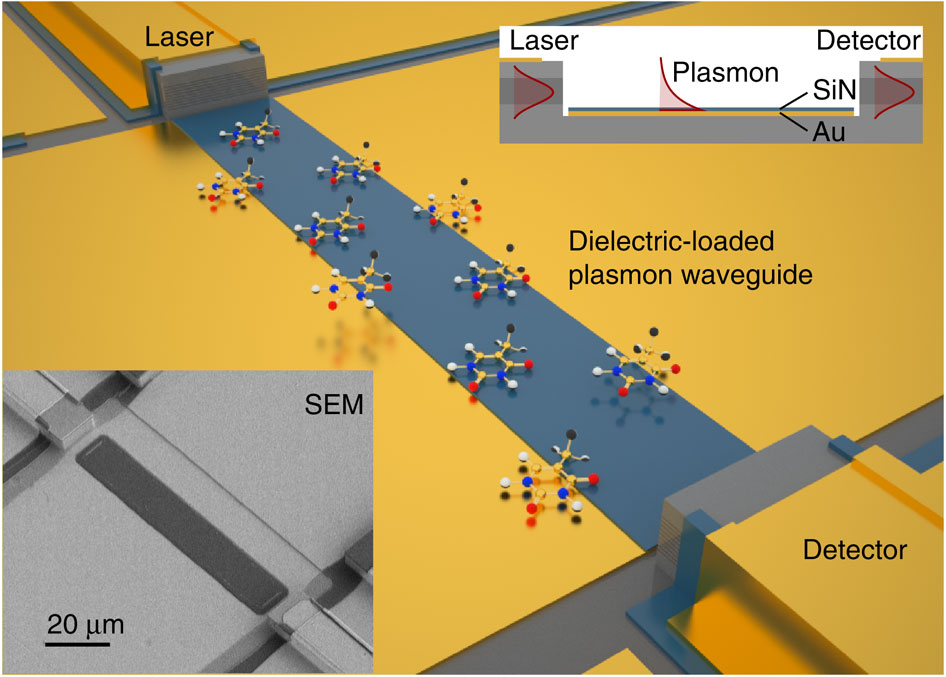
\includegraphics[width=\textwidth]{figures/mlh/laserchip.jpg}
	\caption{Nanoscale chemical sensor, comprised of a laser, a SPP waveguide and a detector, monolithically integrated on the same substrate. The upper inset shows the cross section of the structure and the lower inset the corresponding scanning electron microscope (SEM) image of the fabricated device.\cite{Schwarz2014}}
	\label{fig:laserchip}
\end{figure}

\paragraph{Movement sensor \cite{Kasas13012015}}
A universal life detection sensor has been developed by Kasas et al. of the École Polytechnique Fédérale de Lausanne, by using a cantilever known, as known from Atomic Force Microscopy, to detect tiny fluctuations, commonly associated with the movement and metabolic activity of cells. The cantilever is essentially a metal beam which can scrape a surface, and if any living organisms get stuck on the cantilever, a laser can detect the tiny vibrations made by metabolic movement. The sensor has been successfully tested with bacteria, yeast, mouse cells, human cells, and plant cells. The unique feature of such sensor is the complete lack of knowledge required about the organism biochemistry. Where other methods rely on the assumption that extraterrestrial life has similar DNA, protein or hydrocarbon chemistry as life on earth, no such assumptions are necessary for this detection method.
\begin{figure}[htb]
	\centering
	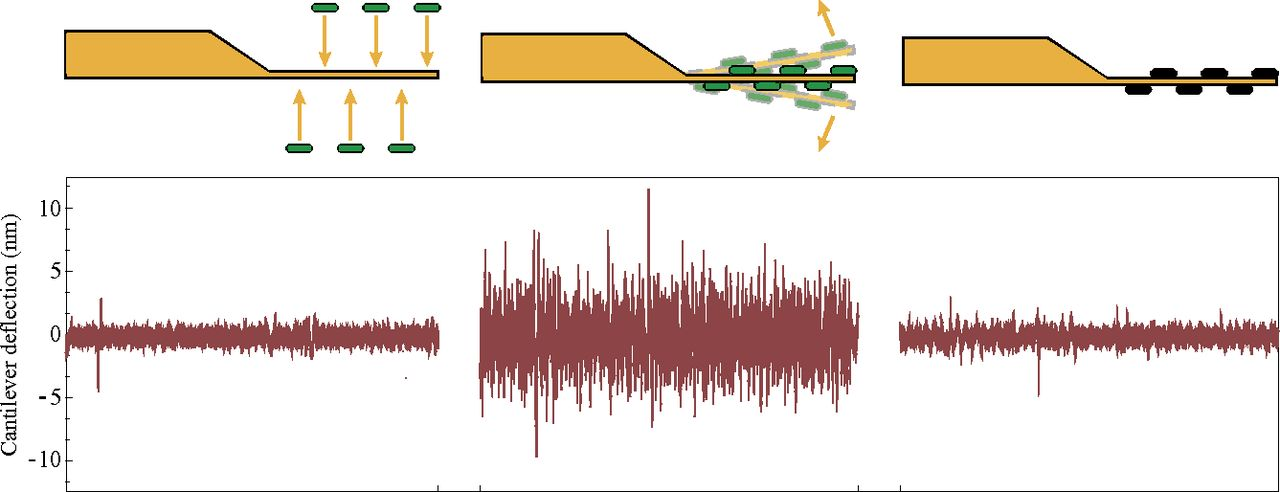
\includegraphics[width=\textwidth]{figures/mlh/movementdetector.jpg}
	\caption{Detailed depiction of a nanomotion detection experiment. Before the attachment of the living specimens to the sensor, the fluctuations are small (Left). When the specimens are immobilized on the sensor, its fluctuations increase (Center). Finally, if the microorganisms are killed, through a chemical or physical agent, the sensor reverts to small fluctuations (Right).}
	\label{fig:movementdetector}
\end{figure}

\paragraph{Wet-chemical analyzers \cite{chemical_microsensors}}
The National Oceanography Centre of the United Kingdom is developing chemical sensors for several of the major nutrients important for oceanic life, which includes nitrate, nitrite, ammonia, and phosphate, as well as the trace nutrients, present at low concentrations yet essential for life, such as dissolved iron and manganese, which is a tracer of hydrothermal vent emissions.  Many of these sensors are based on the principle of Flow Injection Analysis, which is commonly used in laboratory equipment, but with the goal of condensing several high precision sensors into a small device which can be used for in-situ deep ocean analysis and monitoring. Such a system is attained by use of microfluidic devices and sensors.
\begin{figure}[htb]
	\centering
	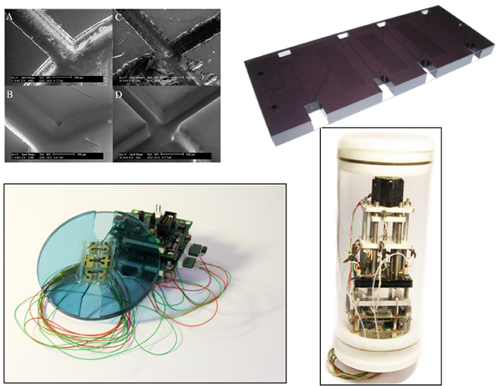
\includegraphics[width=\textwidth]{figures/mlh/microsensors_chem_img1.png}
	\caption{Clockwise from top left: An electron micrograph of four steps in the processing of micro-machined flow channels in a polymer base using a patented process developed at Southampton; a functional microfluidic sensor ‘chip’; a sensor ‘chip’ with its support electronics; finally the senor and electronics, with flow control valves and a pump for the sample and reagent chemicals enclosed within a pressure housing ready to be used at sea.\cite{chemical_microsensors}}
	\label{fig:chemical_microsensors}
\end{figure}

\subsubsection{Implementation}
Although lab-on-a-chip systems and microscopic sensors offer promising products and technologies, many of the applications which are of interest to this mission, are still in a developmental stage, and require further maturing before an extraterrestrial mission can rely on such equipment. The long life of the mission and single-use chips also hinders the effective use of such systems, and it was therefore chosen not to bring LOCs on the Europa subsea mission.

\autsection{Salinity \& pH Sensor}{Kristian Sloth Lauszus and Lukas Christensen}

As previously noted, the pH and salinity of an environment is believed to play a large part in the formation of life. Therefore, sensors able to measure these quantities are an integral part of the instrument contingency of this mission. 

\subsection{Theory}
There exists multiple ways to perform electronic measurements of pH and salinity, however, most of them follow the same basic principle and are more or less variations of the Ion-Selective Electrode (ICE).\\

\noindent
The ICE works by having an electrode (the Ion-Selective Electrode) wrapped in a semi-permeable membrane submerged into the solution to be tested. The membrane is designed such that only ions of a single type, for example H$^+$, is able to penetrate it. When the chosen ion is present in the solution it will start to diffuse through membrane causing a build up of electrical potential across the it. In order to measure this potential difference another electrode, referred to as the reference electrode, is also placed into the solution as shown in figure \ref{fig:iseSchematic}. \\

\begin{figure}[htb]
	\centering
	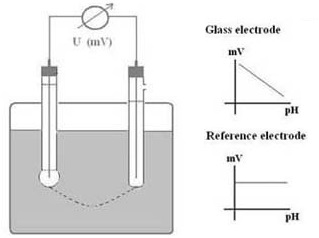
\includegraphics[width=.6\textwidth]{figures/LAMC/iseSchematic}
	\caption{Basic schematic of an Ion-Selective Electrode pH measurement setup. The left is the sensing electrode and the right is the reference. Adapted from \cite{website:ph2}.}
	\label{fig:iseSchematic}
\end{figure}

\noindent
By measuring the voltage across the electrodes the activity of the ion can be determined by the Nernst equation\cite{website:ph1}:
\begin{equation}\label{key}
E = E_0 + 2.303 \frac{R T}{n F} \log_{10}{(A)}
\end{equation}
Where $E$ is the measured potential, $E_0$ is a constant offset that depends on the exact construction of the two electrodes, $R$ is the universal gas constant, $T$ is the temperature, $n$ is the charge of ion to be measured, $F$ is the Faraday constant, and $A$ is the activity of the ion\cite{website:ph1}. As can be seen, the voltage varies linearly with the logarithm of $A$. This makes the ICE extremely well suited for pH-measurements, as the pH is directly proportional to the voltage, meaning only very simple data processing is needed.\\


\noindent
This seemingly simple setup is complicated by the fact that the reference electrode must be in electrical contact with the solution, without causing chemical reactions affecting the potential difference. The way this is most commonly accomplished is by having the reference electrode immersed in an electrolyte with a neutral pH that is separated from the solution to be measured by a membrane\cite{website:ph2}. A common issue with this is that the electrolyte will slowly leak out over time, meaning that the lifetime of an ICE is somewhat limited. \\

\begin{figure}[htb]
	\centering
	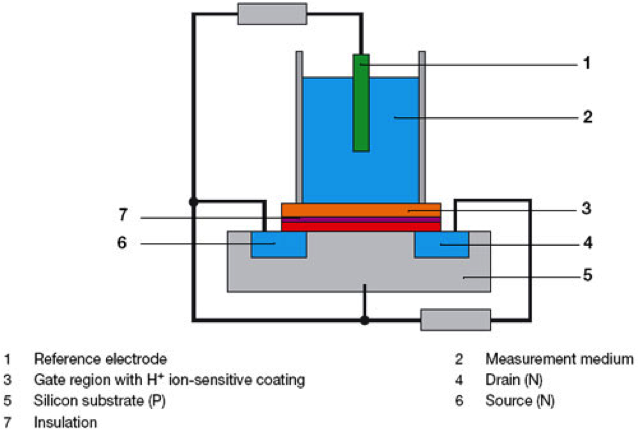
\includegraphics[width=.7\textwidth]{figures/ISFET.png}
	\caption{Schematic of an Ion-Selective Field Effect Transistor. Source: \url{http://www.jumo.de/products/liquid-analysis/ph/electrodes/201050/isfet-ph-single-rod-electrode-201050.html}}
	\label{fig:ISFET}
\end{figure}

\noindent
There are also a host of other issues associated with this type of measurements: To measure the potential difference, a very high impedance sensor is needed as the electrical resistance between the electrodes is commonly in the mega-ohm range\cite{website:ph3}. Furthermore, as can be seen from the Nernst equation, the temperature must be well known to make accurate measurements. Another issue is that the standard way to construct the ion-selective electrode is to have a metal conductor inside a glass bulb filled with an electrolyte, making the sensor fairly fragile. They also require frequent calibration and the membranes that are used to separate different ion-species are very difficult to construct in such a way that only one types of ion makes it through\cite{website:ph1}.\\

\noindent
The fragility and high impedance can be mitigated by the use of Ion-Selective Field Effect Transistors (ISFET). These consists of ordinary FETs but where the gate has been replaced with an ion-sensitive membrane as illustrated in figure \ref{fig:ISFET}. This means that if the sought-for ions are present in a sample that is brought to contact with the ISFET, it will start to conduct electricity proportional to the ion activity. The ISFET then acts as an amplifier and sensor simultaneously, simplifying the signal processing\cite{website:ph4}. Also, even though the membrane is made from a fragile material, such as glass, because only a small piece of it is needed for the gate, the ISFET can be made very durable with performances comparable to more classical methods\cite{website:ph4}. \\ 

\noindent
Other more exotic devices for pH and salinity measurement exist, such as for example voltammetry\cite{website:senova} and holography\cite{article:marshall2003a} based ones. While these devices show great promise and are able to overcome some of the issues associated with ICEs, they are still in their infancy compared to the extremely well characterized ICE systems. Because of this, as well as the fact that they have successfully been used in space before\cite{article:jgre2487}, the ICE provides a very robust solution.

\subsection{Implementation}
The initial sketch of the pH and salinity sensing system for this mission is inspired by the MECA Wet Chemistry Lab on the Phoenix Mars Scout Lander. The Phoenix mission used a number of ICE sensors with different membranes to measure pH and the abundance of various ions in Martian soil\cite{article:jgre2487}. The exact number and nature of the ions to be detected on Europa is beyond the scope of this report, as it would require experts with detailed knowledge in planetary physics and biochemistry in order to select the specific ions that will have the most scientific value. However, pH sensing shall no doubt be included, and the basic sensor design can easily be extended to host an almost arbitrary number of sub-sensors.

\subsection{Discussion}

It has been chosen, contrary to the Phoenix mission, to use ISFETs to form the basis of the sensing element. The reason for this is that these can be made very small, and since they are solid state devices they should easily be able to withstand the very high pressure that can be expected below the Europan ice sheet.\\

\noindent
Furthermore their exist sensors based on this techonology that requires no user calibration\cite{website:senova}. Which would simplify the instrument a lot. The sensors could simply be placed inside the penetrator having the water run by them similar to the approach described in \ref{sec:water_convection}, thus the pH and salinity could be measured contentiously during the entire descent with little effort and take up almost no volume and mass.


\autsection{Camera}{Bhaaeddin Alhomsi}

The cameras will be triggered whenever a detects a flash of light, hopefully catching a glimpse of something living. CMOS camera sensor can detect the wavelength from 350 nm (UVA) till 1100 nm (IRA), so we have to find lighting source can cover this range .
Another approach that is developing very well is that of broad band fluorescence to very deep (short wavelength) ultraviolet (UV) light. The deep UV has the advantage that at such wavelengths there is very little background fluorescence, and it is easy to identify samples containing carbon-based chemistry that could be associated with life.
Infra-red light is radiated from any object with a temperature. Even objects which are too cool to be detected optically can be studied in the infra-red.
Panoramic image (360 degree) it will give us a good understanding how is the bottom of ice shield looks like.

\subsection{Lighting}

Ambient visible light is quickly attenuated by a combination of scattering and absorption, thus requiring artificial lighting to view items underwater with any degree of clarity. We see things in color because objects reflect wavelengths of light that represent the colors of the visible spectrum. Artificial lighting is therefore necessary near the illuminated object to view it in true color with intensity. Underwater lamps provide this capability.
Lamps convert electrical energy into light. The main types or classes of artificial lamps/light sources used in underwater lighting are incandescent, fluorescent, high intensity gas discharge, and light-emitting diode (LED) - each with its strengths and weaknesses. All types of light are meant to augment the natural light present in the environment.
 The flash lamps provide a short duration (about 0.005 see) heat pulse. The short burst of energy results in a momentary rise in the surface temperature of the part. The temperature rise may be detrimental to the top layer of the part being exposed. Therefore, it is necessary to ensure the non-destructive nature of the technique. Amount of the temperature rise determines whether the flash-lamp heating would be detrimental to the part. 
the flash duration is about 0.005 sec. Because of the short flash duration, relatively little amount of heat is imparted. The part temperature on the surface rises until end of the flash duration and then drops quickly due to the heat radiation and convection from the surface and the heat conduction into the part. The temperature rise on the part surface can be high enough to damage the top layer of the part.
The table below, shows the major types of artificial lighting systems, as well as their respective characteristics.
\begin{figure}[htb]
\centering
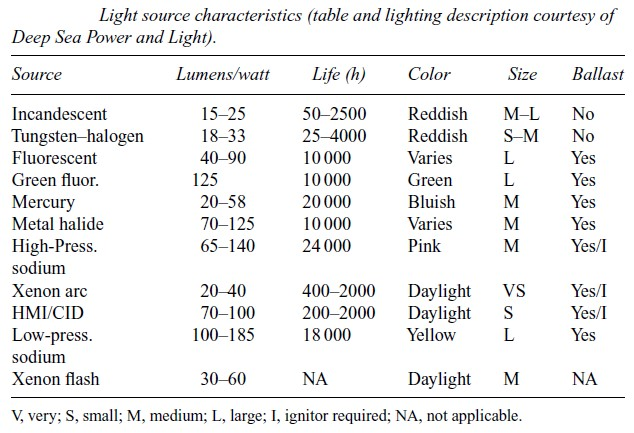
\includegraphics[scale=0.75]{figures/camera/bh6.jpg}
\caption{Light source characteristics}
\end{figure}
\\
Incandescent – The incandescent lamp was the first artificial light bulb invented.
Electricity is passed through a thin metal element, heating it to a high enough temperature to glow (thus producing light). It is inefficient as a lighting source with approximately 90 \% of the energy wasted as heat. Halogen bulbs are an improved incandescent. Light energy output is about 15 \% of energy input,  instead of 10 \%, allowing them to produce about 50 \% more light from the same amount of electrical power. However, the halogen bulb capsule is under high pressure instead of a vacuum or low-pressure noble gas (as with regular
incandescent lamps) and, although much smaller, its hotter filament temperature causes the bulbs to have a very hot surface. This means that such glass bulbs can explode if broken, or if operated with residue (such as fingerprints) on them. The risk of burns or fire is also greater than other bulbs, leading to their prohibition in
some underwater applications. Halogen capsules can be put inside regular bulbs or dichroic reflectors, either for aesthetics or for safety. Good halogen bulbs produce a sunshine-like white light, while regular incandescent bulbs produce a light between sunlight and candlelight.

\begin{figure}[htb]
\centering
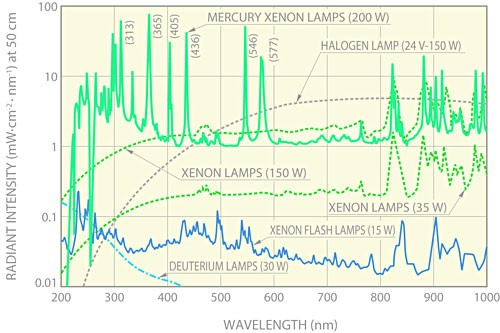
\includegraphics[scale=1]{figures/camera/bh7.jpg}
\caption{Lamp wavelength}
\end{figure}

A fluorescent lamp is a type of lamp that uses electricity to excite
mercury vapour in argon or neon gas, producing short-wave ultraviolet light. This light then causes a phosphor coating on the light tube to fluoresce, producing visible light. Fluorescent bulbs are about 40 \% efficient, meaning that for the same amount of light they use one-fourth the power and produce one-sixth the heat of a regular incandescent. Fluorescents typically do not have the luminescent output capacity per unit volume of other types of lighting, making them (in many underwater applications) a poor choice for underwater artificial light sources.

High-intensity discharge – High-intensity discharge (HID) lamps include the
following types of electrical lights: Mercury vapour, metal halide, high pressure sodium and, less common, xenon short-arc lamps. The light-producing element of these lamp types is a well-stabilized arc discharge contained within a refractory envelope (arc tube) with wall loading (power intensity per unit area of the arc tube) in excess of 3W/cm2 (19.4 W/in2). Compared to fluorescent and incandescent lamps, HID lamps produce a large quantity of light in a small package, making them well suited for mounting on underwater vehicles. The most common HID lights used in underwater work are of the metal halide type.

LED – A light-emitting diode (LED) is a semiconductor device that emits incoherent narrow-spectrum light when electrically biased in the forward direction. This effect is a form of electroluminescence. The color of the emitted light depends on the chemical composition of the semiconducting material used, and can be near-ultraviolet, visible, or infra-red. LED technology is useful for underwater lighting because of its low power consumption, low heat generation, instantaneous on/off control, continuity of color throughout the life of the diode, extremely long life, and relatively low cost of manufacture. LED lighting is a rapidly evolving technology \cite{lighting}.

We will select xenon lamp 150 W, because it will provide us with good radiant intensity for the whole wavelength range.

\subsection{Reflector}
An efficient reflector will not only maximize the light output that falls on the target, but will also direct heat forward and away from the lamp. The shape of the reflector will be the main determinant in how the light output is directed. Most are parabolic, but ellipsoidal reflectors are often used in underwater applications to focus light through a small opening in a pressure housing. 

The surface condition of a reflector
will determine how the light output will be dispersed and diffused. The majority of reflectors are made of pure, highly polished aluminium that will reflect light back at roughly the same angle to the normal at which it was incident. By adding dimples or peens to the surface, the reflected light is dispersed or spread out. When a plain white surface is used, the reflected light is diffused in all directions.

\subsection{The wavelength range of optical radiation}

The term "optical radiation" refers to electromagnetic radiation in the wavelength range between 100 nm and 1 mm. The terms "light" and "visible radiation" (VIS) refer to the wavelength range between 400 nm and 800 nm, which can be perceived by the human eye. Optical radiation with wavelengths shorter than 400 nm is called ultraviolet (UV) radiation and is further subdivided in UV-A, UV-B and UV-C ranges. Similarly, infra-red (IR) radiation covers the wavelength range above 800 nm and is subdivided in IR-A, IR-B and IR-C ranges.

\begin{figure}[htb]
\centering
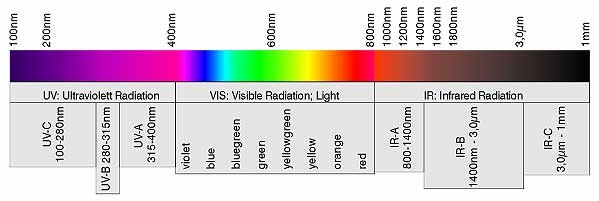
\includegraphics[scale=1]{figures/camera/bh8.jpg}
\caption{The wavelength range of optical radiation}
\end{figure}

The sensitivity of the human eye to light of a certain intensity varies strongly over the wavelength range between 380 and 800 nm. Under daylight conditions, the average normal sighted human eye is most sensitive at a wavelength of 555 nm.

\subsection{Camera}

The ECAM imaging system delivers cost-effective, short lead-time, high-performance, and reliable space imaging as a modular off-the-shelf solution. The C50 utilizes a CMOS image sensor with integral RGB Bayer Pattern color filter array. The sensor outputs 10-bit pixels that are square-root companded to 8-bits before being transmitted to the DVR on a 200 Mbit/s serial link.. Preprocessing typically includes Bayer Pattern interpolation and direct conversion to the YCbCr color space using a 5 x 5 filter kernel. The video is also reformatted as needed for input to either a JPEG (lossy) or Huffman First Difference (lossless) compressor. The C50 is highly configurable. The exposure and gain may be adjusted to support widely varying scene. The optical lens made of a material that has substantially the same index of refraction as that of water.$http://www.msss.com/brochures/c50.pdf$

\begin{figure}[htb]
\centering
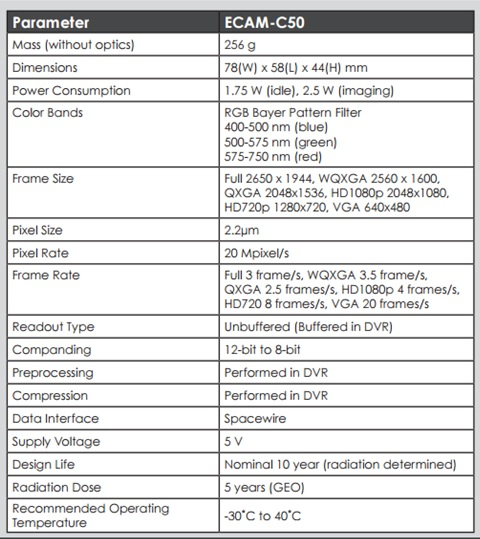
\includegraphics[width=.48\textwidth]{figures/camera/bh10.jpg}
\caption{Camera parameters}
\end{figure}

CMOS sensor can detect the wavelength from 350 nm (UVA) till 1100 nm (IRA), so we have to find lighting source can cover this range .

\begin{figure}[htb]
\centering
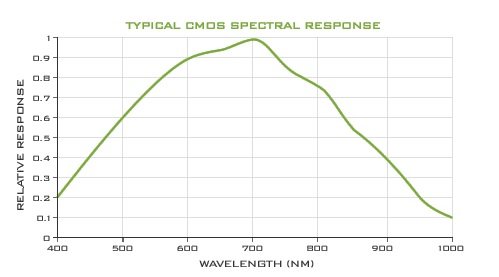
\includegraphics[scale=1]{figures/camera/bh9.jpg}
\caption{CMOS spectral response}
\end{figure}

\subsection{Panoramic Images}

To take a panorama, the camera is rotated at fixed angular increments, taking an image at each point. These images can then be assembled (stitched) using stitching software, which allows the images to be aligned and combined into a single seamless panoramic image, either automatically (using image analysis) or manually (with user supplied control points).For this mission we will fix the camera on the robotic arm, and the arm will rotate and taking images. These images will sent to the earth. In the earth, the images aligned and combined into panoramic image.
The rotation angle depend on camera field of view , in or proposed camera the field of view angle is approximately 70 degree , so to build 360 panoramic image we need 5 photos with rotation angle 70 degree between each shoot.


\section{Microscope}
